\documentclass[a4paper]{article}

%Tutti gli usepackage vanno qui

\usepackage{geometry}
\usepackage[italian]{babel}
\usepackage[utf8]{inputenc}
\usepackage[T1]{fontenc}
\usepackage{tabularx}
\usepackage{longtable}
\usepackage{hyperref}
\usepackage{enumitem}
\hypersetup{
	colorlinks=true,
	linkcolor=black,
	filecolor=magenta,      
	urlcolor=blue,
}
% Numerazione figure 
\let\counterwithout\relax
\let\counterwithin\relax
\usepackage{chngcntr}

\counterwithin{table}{subsection}
\counterwithin{figure}{subsection}

\usepackage[bottom]{footmisc}
\usepackage{fancyhdr}
\usepackage{titlesec}
\setcounter{secnumdepth}{4}
\usepackage{amsmath, amssymb}
\usepackage{array}
\usepackage{graphicx}

%\usepackage{float}
\usepackage{layouts}
\usepackage{float}
\usepackage{eurosym}


\usepackage{layouts}
\usepackage{float}
\usepackage{eurosym}

%Comandi di impaginazione uguale per tutti i documenti
\pagestyle{fancy}
\lhead{
\includegraphics[scale=0.07]{res/images/logo8_crop.png}}
%Titolo del documento
\rhead{\doctitle{}}
\rfoot{\thepage}
\cfoot{}
\setlength{\headheight}{35pt}
\setcounter{tocdepth}{4}
\setcounter{secnumdepth}{4}
\renewcommand{\footrulewidth}{0.4pt}

% multirow per tabelle
\usepackage{multirow}

% Permette tabelle su più pagine

%\usepackage{longtable}


% colore di sfondo per le celle
\usepackage[table]{xcolor}

%COMANDI TABELLE
\newcommand{\rowcolorhead}{\rowcolor[HTML]{56A5EC}} %intestazione 
\newcommand{\rowcolorlight}{\rowcolor[HTML]{fafafa}} %righe chiare/dispari
\newcommand{\rowcolordark}{\rowcolor[HTML]{e1f5fe}} %righe scure/pari
\newcommand{\colorhead}{\color[HTML]{FFFFFF}} %testo intestazione
\newcommand{\colorbody}{\color[HTML]{000000}} %testo righe
\newcommand{\tabitem}{~~\rlap{\textbullet}~~}

\newcommand{\glo}{$_{G}$}
\newcommand{\glosp}{$_{G}$ }

\definecolor{pari}{HTML}{E1F5
\definecolor{dispari}{HTML}{FAFAFA}


%Lista dei comandi personalizzati
\newcommand{\doctitle}{Verbale interno 2019-02-20}
\newcommand{\rev}{1.0.0}
\newcommand{\approv}{}
\newcommand{\ver}{}
\newcommand{\red}{Matteo Santinon}
\newcommand{\stato}{Approvato}
\newcommand{\uso}{Interno}
\newcommand{\describedoc}{Riassunto dell'incontro del gruppo \textit{8Lab 
Solutions} tenutosi il 2019-02-20.}
\newcommand{\destinatari}{8Lab Solutions\\& Prof. Tullio Vardanega\\& Prof. Riccardo Cardin}



\makeindex

\usepackage{hyperref}	%queste due linee le ho aggiunte altrimenti non funzionano i link


\begin{document}
	\thispagestyle{empty}
\begin{titlepage}
	\begin{center}
		
\includegraphics[scale = 0.3]{res/images/logo8_crop.png}\\
		\large \textbf{8Lab Solutions - Progetto "Soldino"} \\
		\vfill
		\Huge \textbf{\doctitle}
		\vspace*{\fill}
        
        \vfill
        \large
        \begin{tabular}{r|l}
                        \textbf{Versione} & \rev{} \\
                        \textbf{Approvazione} & \approv{} \\
                        \textbf{Redazione} & \red{} \\
                        \textbf{Verifica} & \ver{} \\
                        \textbf{Stato} & \stato{} \\
                        \textbf{Uso} & \uso{} \\
                        \textbf{Destinato a} & \parbox[t]{5cm}{8Lab Solutions
                        \\Prof. Tullio Vardanega\\Prof. Riccardo Cardin}
                \end{tabular}
                \vfill
                \normalsize
                \textbf{Descrizione}\\
                \describedoc
                \vfill
                \small
                \texttt{8labsolutions@gmail.com}
	\end{center}
\end{titlepage}

	\pagebreak	
	
	\section*{Changelog}
\renewcommand{\arraystretch}{1.5}
\rowcolors{2}{pari}{dispari}
	\begin{longtable}{ 
			>{\centering}p{0.09\textwidth} 
			>{\centering}p{0.13\textwidth}
			>{\centering}p{0.2\textwidth} 
			>{\centering}p{0.16\textwidth} 
			>{}p{0.2775\textwidth} }
		
		\rowcolorhead
		\textbf{\color{white}Version} & 
		\textbf{\color{white}Date} & 
		\textbf{\color{white}Name} & 
		\textbf{\color{white}Role} &
		\centering \textbf{\color{white}Description} 
		\tabularnewline  
		\endfirsthead
		\rowcolorhead
		\textbf{\color{white}Version} & 
		\textbf{\color{white}Date} & 
		\textbf{\color{white}Name} & 
		\textbf{\color{white}Role} &
		\centering \textbf{\color{white}Description} 
		\tabularnewline  
		\endhead
		
		1.0.0 & 2019-03-30 & PLACEHOLDER & \textbf{Project Manager} &
		Approval
		\tabularnewline
		
		0.2.0 & 2019-03-27 & PLACEHOLDER & \textbf{Verifier} &
		Verification
		\tabularnewline
		
		0.1.2 & 2019-03-25 & PLACEHOLDER & \textbf{RUOLO} &
		Written §5.3, §5.4 and §6
		\tabularnewline
		
		0.1.2 & 2019-03-25 & PLACEHOLDER & \textbf{RUOLO} &
		Written §4.4 and §4.5
		\tabularnewline
		
		0.1.1 & 2019-03-24 & PLACEHOLDER & \textbf{RUOLO} &
		Written §3.3 and §4.3
		\tabularnewline
		
		0.1.0 & 2019-03-22 & PLACEHOLDER & \textbf{Verifier} &
		Verification
		\tabularnewline
		
		0.0.4 & 2019-03-21 & PLACEHOLDER & \textbf{RUOLO} &
		Written §3.2, §4.2 and §5.2
		\tabularnewline
		
		0.0.3 & 2019-03-21 & PLACEHOLDER & \textbf{RUOLO} &
		Written §3.1, §4.1 and §5.1
		\tabularnewline
		
		0.0.2 & 2019-03-20 & PLACEHOLDER & \textbf{RUOLO} &
		Written §1 and §2
		\tabularnewline
		
		0.0.1 & 2019-03-20 & Federico Bicciato & 
		\textbf{RUOLO} & Created document's structure.
		\tabularnewline
		
	
	\end{longtable}
\renewcommand{\arraystretch}{1} 


	\counterwithin{table}{subsection}
	\counterwithin{figure}{subsection}
	\pagebreak
	
	\tableofcontents
	\pagebreak
	
	\listoffigures
	\pagebreak
	
	\listoftables
	\pagebreak
	
	\section{Introduzione}
\subsection{Scopo del documento}
Questo documento ha lo scopo di definire delle regole di base che tutti i membri 
di \textit{8Lab Solutions} devono rispettare nello svolgimento del progetto, 
così da garantire uniformità in tutto il materiale. Verrà utilizzato un 
approccio incrementale, volto a normare passo passo ogni decisione discussa e 
concordata tra tutti i membri del gruppo. Ciascun componente è obbligato a 
prendere visione di tale documento e a rispettare le norme in esso descritte 
allo scopo di perseguire la coesione\glosp all'interno del team.

\subsection{Scopo del prodotto}
Il capitolato\glosp C6 ha per obiettivo lo sviluppo di una piattaforma chiamata \textit{Soldino} che è basata sull'infrastruttura Ethereum\glo{} e funzionante tramite il meccanismo degli smart contracts\glo{}. \textit{Soldino} è gestita dal governo\glosp e ha lo scopo di assistere le aziende nella gestione dell'IVA riguardo tutte le operazioni di compravendita di beni e servizi. Il governo può coniare e 
distribuire la moneta utilizzata in queste transazioni, mentre i cittadini 
potranno acquistare i beni utilizzando tale valuta. La piattaforma, dunque, 
intende divenire un punto di incontro tra governo, aziende e cittadini.

\subsection{Glossario}
Al fine di evitare possibili ambiguità relative al linguaggio utilizzato nei documenti formali, viene fornito il \textit{Glossario v2.0.0}. In questo documento vengono definiti e descritti tutti i termini con un significato particolare. Per facilitare la lettura, i termini saranno contrassegnati da una 'G' a pedice.

\subsection{Riferimenti}
\subsubsection{Riferimenti normativi}
\begin{itemize}

	\item \textbf{Capitolato d'appalto C6 - Soldino, piattaforma Ethereum per pagamenti IVA}: \\
		\url{https://www.math.unipd.it/~tullio/IS-1/2018/Progetto/C6.pdf};
%verbali normativi PLACEHOLDER
\end{itemize}

\subsubsection{Riferimenti informativi}
\begin{itemize}
	\item \textbf{ Standard ISO/IEC 12207:1995}:\\* 
	\url{https://www.math.unipd.it/~tullio/IS-1/2009/Approfondimenti/ISO_12207-1995.pdf};
	\item \textbf{La qualità secondo ISO/IEC 9126}: \\*
	\url{http://www.colonese.it/00-Manuali_Pubblicatii/07-ISO-IEC9126_v2.pdf};
	\item \textbf{Slide L05 del corso Ingegneria del Software - Ciclo di vita 
	del software}:\\
		\url{https://www.math.unipd.it/~tullio/IS-1/2016/Dispense/L05.pdf};
	\item \textbf{Guide to the Software Engineering Body of Knowledge(SWEBOK), 2004} \\*
		\url{http://www.math.unipd.it/~	tullio/IS-1/2007/Approfondimenti/SWEBOK.pdf};
	\item \textbf{Software Engineering - Ian Sommerville - 9 th Edition (2010)}: \\*
		(formato cartaceo);
	\item \textbf{Documentazione git}: \\*
		\url{https://www.atlassian.com/git};
	\item \textbf{Standard ISO 8601}: \\*
		\url{https://it.wikipedia.org/wiki/ISO_8601}
	\item \textbf{Snake Case}\glo: \\*
		\url{https://it.wikipedia.org/wiki/Snake_case}
	\item \textbf{Airbnb JavaScript style guide}: \\*
		\url{https://github.com/airbnb/javascript/blob/master/README.md}
	
	
	
	
\end{itemize}

	\pagebreak
	
	\section{Processi primari}

\subsection{Fornitura}

\subsubsection{Scopo}
Lo scopo del processo di fornitura è di determinare le procedure e le risorse 
necessarie allo svolgimento del progetto. Una volta comprese le richieste del 
proponente e aver stilato uno \textit{Studio di Fattibilità}, il processo può 
essere avviato con fine di soddisfare ognuna di queste richieste. Inoltre si 
deve stipulare e concordare con il proponente un contratto per la consegna del 
prodotto. Si passa dunque a determinare le procedure, le risorse necessarie, e 
si sviluppa un \textit{Piano di Progetto} che getterà le basi da perseguire fino 
alla consegna del materiale prodotto.
Il processo di fornitura è composto dalle seguenti fasi:
	\begin{itemize}
		\item avvio;
		\item approntamento di risposte alle richieste;
		\item contrattazione;
		\item pianificazione;
		\item esecuzione e controllo;
		\item revisione e valutazione;
		\item consegna e completamento.
	\end{itemize}
	
\paragraph{Aspettative} \mbox{}\\ 

\noindent Il gruppo intende mantenere un costante dialogo con il proponente, per avere un 
riscontro efficace sul lavoro svolto e instaurare un rapporto di collaborazione 
per quanto riguarda:
	\begin{itemize}
		\item determinare aspetti chiave per far fronte ai bisogni del proponente;
		\item stilare requisiti e vincoli sui processi;
		\item stimare le tempistiche di lavoro;
		\item promuovere una verifica continua;
		\item chiarire eventuali dubbi emersi;
		\item accordarsi sulla qualifica del prodotto.
	\end{itemize}
	
\paragraph{Descrizione} \mbox{}\\ 

\noindent Questa sezione tratta le norme che i membri del gruppo \textit{8Lab Solutions} 
devono rispettare in tutte le fasi di progettazione, sviluppo e consegna del 
prodotto \textit{Soldino}, al fine di diventare fornitori nei confronti del 
proponente \textit{Red Babel} e dei committenti Prof. Tullio Vardanega e Prof. 
Riccardo Cardin.

\subsubsection{Attività}

\paragraph{Studio di Fattibilità} \mbox{}\\ 

\noindent \'E compito del responsabile di progetto organizzare riunioni tra i membri del 
gruppo al fine di permettere lo scambio di opinioni sui capitolati proposti.
Lo \textit{Studio di Fattibilità}, redatto dagli analisti, indica per ogni 
capitolato\glo:
	\begin{itemize}
		\item \textbf{informazioni generali}: vengono elencate le informazioni di 
			base, come il nome del progetto, il proponente e il committente;
		\item \textbf{descrizione e finalità del progetto}: viene fatta una 
			presentazione del capitolato\glosp in generale, una descrizione delle 
			caratteristiche principali richieste per il prodotto e viene definito 
			l'obiettivo che si vuole raggiungere;
		\item \textbf{tecnologie interessate}: viene fatto un elenco delle tecnologie 
			richieste per lo svolgimento, che rientrano nel dominio tecnologico;
		\item \textbf{aspetti positivi, criticità e fattori di rischio}: vengono 
			esposte le considerazione fatte dal gruppo sugli aspetti positivi e sui fattori 
			di rischio del capitolato\glo;
		\item \textbf{conclusioni}: vengono esposte le ragioni per la quale il gruppo 
			ha deciso di accettare o scartare il capitolato\glo.
	\end{itemize}
		
\paragraph{Piano di Progetto} \mbox{}\\ 

\noindent Il responsabile, con l'aiuto degli amministratori, redige un \textit{Piano di 
Progetto} da seguire durante il corso del progetto. Questo documento contiene:
	\begin{itemize}
		\item \textbf{analisi dei rischi}: vengono analizzati nel dettaglio i rischi 
			che potranno presentarsi e vengono esposte le misure e le modalità attraverso le 
			quali i rischi vengono contenuti o mitigati. Viene anche fornita la probabilità 
			con la quale questi possono presentarsi e il livello di gravità per ciascuno;
		\item \textbf{modello di sviluppo\glo}: viene descritto il modello di 
			sviluppo\glosp che è stato scelto, indispensabile per la pianificazione;
		\item \textbf{pianificazione}: vengono pianificate le attività da eseguire 
			nelle diverse fasi del progetto e vengono stabilite le loro scadenze temporali;
		\item \textbf{preventivo e consuntivo}: viene data una stima di lavoro 
			necessaria per ciascuna fase proponendo così un preventivo per il costo totale 
			del progetto. Viene anche tracciato, un consuntivo di periodo relativo 
			all'andamento rispetto a ciò che è stato preventivato.
	\end{itemize}
		
\paragraph{Piano di Qualifica} \mbox{}\\

\noindent I verificatori dovranno redigere un documento, detto \textit{Piano di 
Qualifica} contenente le strategie da adottare per garantire la qualità del 
materiale prodotto dal gruppo, e dei processi attuati. Il piano è così 
suddiviso:
	\begin{itemize}
		\item \textbf{qualità di processo}: vengono identificati dei processi dagli 
			standard, stabiliti degli obiettivi, escogitate delle strategie per attuarli e 			
			individuate le metriche per misurarli e controllarli;
		\item \textbf{qualità di prodotto}: vengono identificati gli attributi più 
			rilevanti per il prodotto, definiti degli obiettivi per raggiungerli e delle 
			metriche per misurarli;
		\item \textbf{specifiche dei test}: definiscono una serie di test attraverso 
			i quali il prodotto passa per garantire che soddisfi i requisiti;
		\item \textbf{standard di qualità}: vengono esposti gli standard di qualità 
			scelti;
		\item \textbf{valutazioni per il miglioramento:} vengono riportati i problemi 
			e le relative soluzioni nel ricoprire un determinato ruolo e nell'uso degli 
			strumenti scelti;
		\item \textbf{resoconto delle attività di verifica:} per ogni attività si 
			riportano i risultati delle metriche calcolate in forma di resoconto.
	\end{itemize}
		
\subsubsection{Strumenti}
Di seguito sono elencati gli strumenti utilizzati durante il processo di 
fornitura.

\paragraph{Microsoft Excel} \mbox{}\\ 

\noindent Software della suite Microsoft Office per realizzare fogli elettronici. Usato 
per fare calcoli, produrre diagrammi, istogrammi e areogrammi, creare tabelle e 
grafici.
		
\paragraph{Microsoft Project} \mbox{}\\ 

\noindent Per assistere i responsabili di progetto nella pianificazione, 
nell'assegnazione delle risorse, nella verifica del rispetto dei tempi, nella 
gestione dei budget e nell'analisi dei carichi di lavoro attraverso la creazioni 
di diagrammi di Gantt\glo, è stato utilizzato Microsoft Project. \\
		\centerline{\url{https://products.office.com/it-it/project/}}
		%PLACEHOLDER
	\begin{figure}[H]
		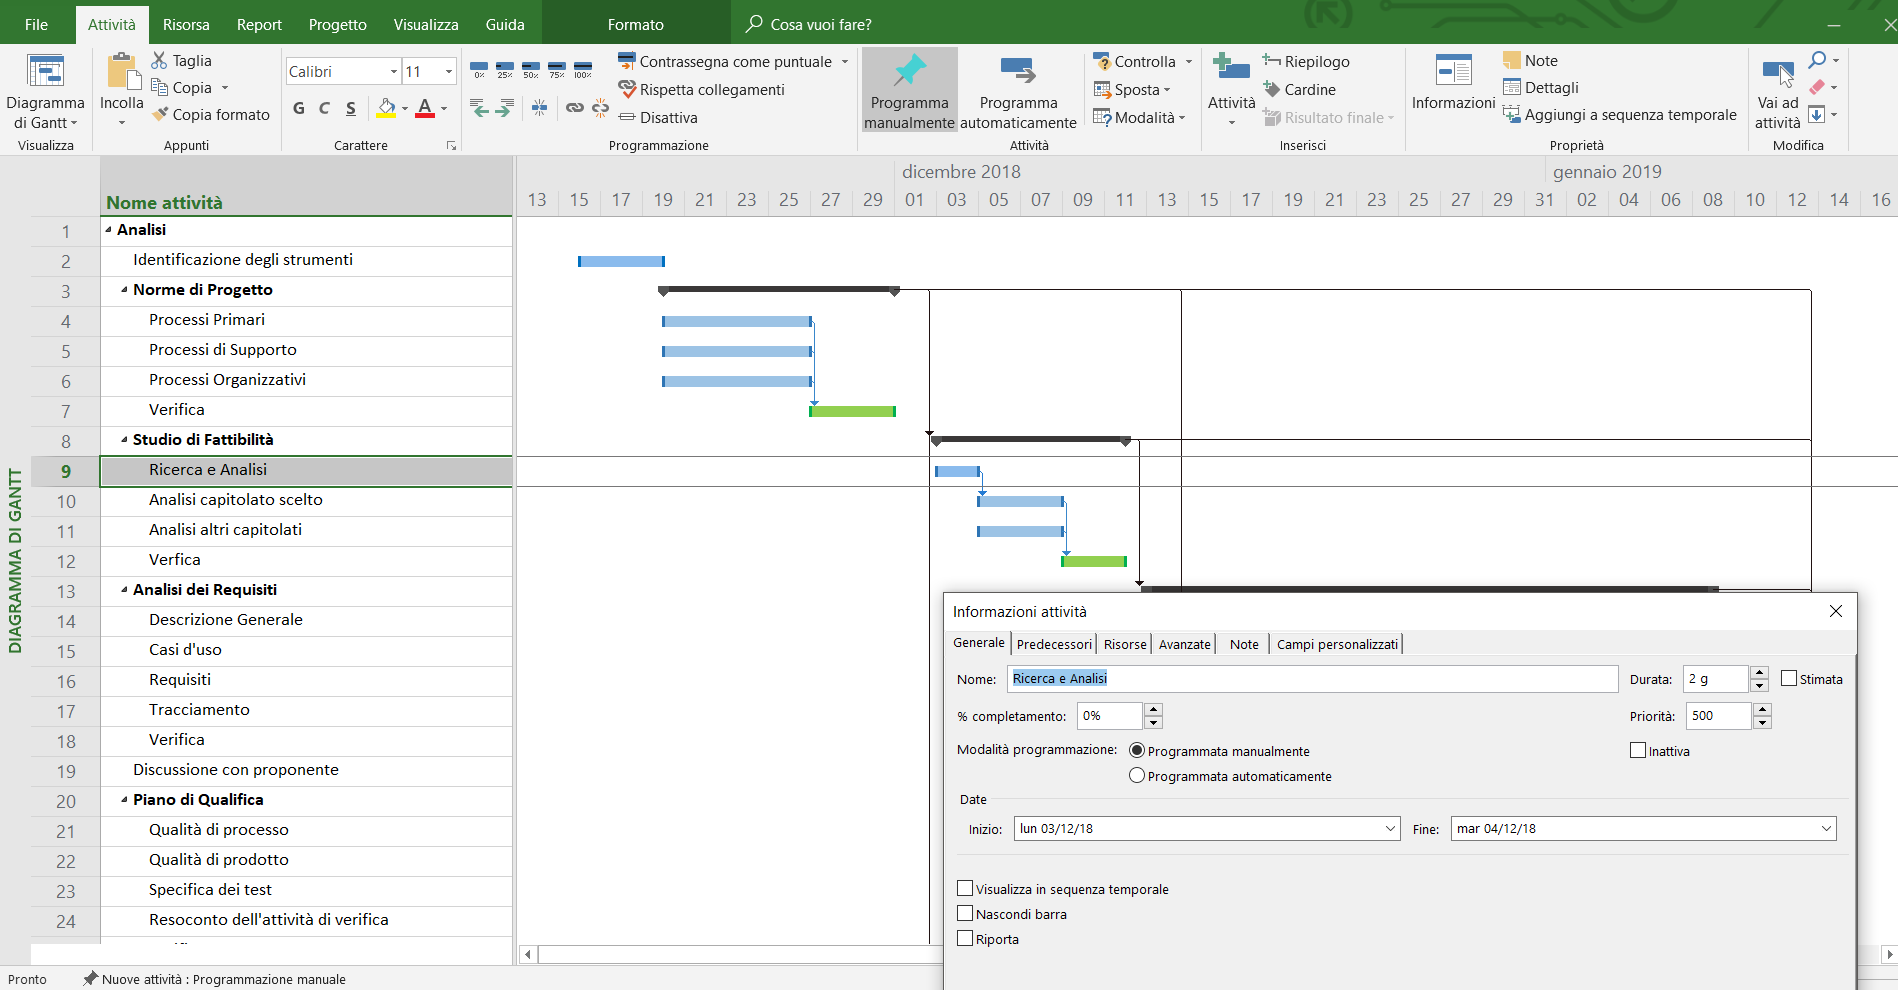
\includegraphics[width=0.99\linewidth]{res/images/projectS.png}
		\caption{Microsoft Project: Gantt}
	\end{figure}
	 

		
%\subsubsection{Collaudo e consegna del prodotto}
%Al fine di consegnare il prodotto terminato il gruppo deve effettuare un 
%collaudo in presenza del proponente e dei committenti. Precedentemente a questo 
%test il gruppo deve assicurare correttezza, completezza e affidabilità per ogni 
%parte del materiale consegnato, permettendo così che tutti i requisiti 
%obbligatori siano soddisfatti e l'esecuzione dei test abbiano un esito positivo. 
%In seguito al collaudo finale il responsabile di progetto consegna il prodotto 
%su un supporto fisico.
		
     
\subsection{Sviluppo}

\subsubsection{Scopo}
Il processo contiene le attività e i compiti da svolgere, al fine di realizzare 
il prodotto finale richiesto dal proponente.

\subsubsection{Aspettative}
Le aspettative sono le seguenti:
	\begin{itemize}
		\item fissare gli obiettivi di sviluppo;
		\item fissare i vincoli tecnologici;
		\item fissare i vincoli di design;
		\item realizzare un prodotto finale che supera i test, che soddisfa i 
			requisiti e le richieste del proponente.
	\end{itemize}
	
\subsubsection{Descrizione}
Il processo di sviluppo si articola in:
	\begin{itemize}
		\item analisi dei requisiti;
		\item progettazione;
		\item codifica.
	\end{itemize}
	
\subsubsection{Attività}
\paragraph{Analisi dei requisiti} 
\paragraph*{Scopo}  \mbox{}\\ 

\noindent Gli analisti individuano i requisiti del progetto attraverso lo studio del 
capitolato, gli incontri con il proponente e i casi d'uso. Tali requisiti sono 
presenti nel documento formale \textit{Analisi dei Requisiti}, in cui viene riportata 
anche la lista dei casi d'uso. \\
Lo scopo dei requisiti è quello di:
	\begin{itemize}
		\item definire la finalità del lavoro;
		\item fornire ai progettisti riferimenti precisi ed affidabili;
		\item fissare le funzionalità e i requisiti concordati col cliente;
		\item fornire  una  base  per  raffinamenti  successivi  al  fine  di  
			garantire  un miglioramento continuo del prodotto e del processo di sviluppo;
		\item fornire ai verificatori riferimenti per l'attività di controllo dei 
			test;
		\item calcolare la mole di lavoro per tracciare dei riferimenti per un stima 
			dei costi.
	\end{itemize}
	
\paragraph*{Aspettative} \mbox{}\\

\noindent Obiettivo dell'attività è la creazione della documentazione formale 
contenente tutti i requisiti richiesti dal proponente.			
\paragraph*{Descrizione} \mbox{}\\

\noindent I requisiti si raccolgono secondo modalità predefinite:
	\begin{itemize}
		\item lettura del capitolato\glo, analisi e approfondimento dello stesso;
		\item confronto con il proponente;
		\item confronto tra membri del team di progetto;
		\item analisi di uno o più casi d'uso.  \\
	\end{itemize}
	

\paragraph*{Classificazione dei casi d'uso} \mbox{}\\

\noindent Ogni caso d'uso viene classificato secondo la seguente notazione: \newline \newline
\centerline{\textbf{UC[codice\_padre].[codice\_figlio]}} \\
Dove:
	\begin{itemize}
		\item \textbf{codice\_padre}: numero che identifica univocamente i casi 
			d'uso;
		\item \textbf{codice\_figlio}: numero progressivo che identifica i 
			sottocasi. Può a sua volta includere altri livelli. \\
	\end{itemize}
			%\pagebreak
			%esempio di caso d'uso?(immagine)
Inoltre per ogni caso d'uso bisogna indicare:
	\begin{itemize}
		\item codice identificativo;
		\item titolo;
		\item diagramma UML\glo;
		\item attori primari;
		\item attori secondari;
		\item descrizione;
		\item scenario principale;
		\item scenario alternativo (se presente);
		\item inclusioni(se presenti);
		\item estensioni(se presenti);
		\item specializzazioni(se presenti);
		\item precondizione;
		\item postcondizione. \\
	\end{itemize}


\paragraph*{Classificazione dei requisiti} \mbox{}\\ \label{sec:UC}

\noindent Ogni requisito viene classificato secondo la seguente notazione: \newline \newline
\centerline{\textbf{R[Importanza][Tipologia][Codice]}} \\ 
Dove:
	\begin{itemize}
		\item \textbf{Importanza}: ogni requisito può assumere uno dei seguenti 
			valori:
			\begin{itemize}
				\item \textit{1}: requisito obbligatorio, ovvero irrinunciabile per gli 
					stakeholder;
				\item \textit{2}: requisito desiderabile, ovvero non strettamente 
					necessari ma a valore aggiunto riconoscibile;
				\item \textit{3}: requisito opzionale, ovvero relativamente utile oppure 
					contrattabile più avanti nel progetto.	
			\end{itemize}
		\item \textbf{Tipologia}: ogni requisito può assumere uno dei seguenti 
			valori:
			\begin{itemize}
				\item \textit{F}: funzionale;
				\item \textit{Q}: prestazionale;
				\item \textit{P}: qualitativo;
				\item \textit{V}: vincolo.
			\end{itemize}
		\item \textbf{Codice}: è un identificatore univoco del requisito in forma 
			gerarchica padre/figlio.
	\end{itemize}
	
\noindent
Inoltre per ogni requisito bisogna indicare:	
	\begin{itemize}		
		\item \textbf{classificazione}: viene riportata l'importanza del requisito. 
			Sebbene questa sia un'informazione ridondante ne facilita la lettura;
		\item \textbf{descrizione}: descrizione breve ma completa del requisito, 
			meno ambigua possibile;
		\item \textbf{fonti}: ogni requisito può derivare da una o più tra le 
		seguenti opzioni:
		\begin{itemize}
			\item \textit{capitolato\glo}: si tratta di un requisito individuato dalla 
				lettura del capitolato\glo;
			\item \textit{interno}: si tratta di un requisito che gli analisti hanno 
				ritenuto opportuno aggiungere;
			\item \textit{caso d'uso}: il requisito è estrapolato da uno o più casi 
				d'uso. In questo caso deve essere riportato il codice univoco del caso d'uso;
			\item \textit{verbale}: si tratta di un requisito individuato in seguito ad 
				una richiesta di chiarimento con il proponente. Tali informazioni sono riportate 
				nei verbali in cui ogni requisito individuato è segnato da un codice presente 
				nella tabella dei tracciamenti. \\
		\end{itemize}
	\end{itemize}

\paragraph*{Diagrammi UML} \mbox{}\\ \label{sec:UML}

\noindent I diagrammi UML\glosp devono essere realizzati usando la versione del 
linguaggio v2.0 e per garantirne la leggibilità è necessario:
	\begin{itemize}
		\item distribuire in modo omogeneo gli elementi e possibilmente allinearli 
			sia in senso verticale che in senso orizzontale;
		\item mantenere i margini di spazio tra gli elementi di un gruppo uguali a 
			quelli di gruppi analoghi qualora si hanno le stesse tipologie di elementi;
		\item impostare i collegamenti in uscita da un elemento ad angolo retto. 
	\end{itemize}

\paragraph{Progettazione} 
\paragraph*{Scopo} \mbox{}\\

\noindent L'attività di progettazione definisce, in funzione dei requisiti specificati 
nel documento \textit{Analisi dei Requisiti}, le caratteristiche del prodotto 
software richiesto. Il compito di questa fase è definire una soluzione del 
problema che sia soddisfacente per tutti gli stakeholder. La progettazione segue 
il procedimento inverso rispetto all'\textit{Analisi dei Requisiti} che divide 
il problema in parti per capirne completamente il dominio applicativo. La 
progettazione, infatti, rimette insieme le parti specificando le funzionalità 
dei sottosistemi in modo da ricondurre ad un'unica possibile soluzione. \newline 


\paragraph*{Aspettative} \mbox{}\\

\noindent Il processo ha come risultato la realizzazione dell'architettura del sistema. 
\newline

\paragraph*{Descrizione}  \mbox{}\\

\noindent Le parti principali sono due:
	\begin{itemize}
		\item \textbf{technology baseline}: contiene le specifiche della 
			progettazione ad alto livello del prodotto e delle sue componenti, l'elenco dei 
			diagrammi UML\glosp che saranno utilizzati per la realizzazione 
			dell'architettura e i test di verifica;
		\item \textbf{product baseline}: dettaglia ulteriormente l'attività di 
			progettazione, integrando ciò che è riportato nella technology baseline. Inoltre 
			definisce i test necessari alla verifica. \newline
	\end{itemize}


\paragraph*{Technology baseline} \mbox{}\\

\noindent Redatta dal progettista, dovrà includere:
	\begin{itemize}
		\item \textbf{diagrammi UML\glo}:
		\begin{itemize}
			\item diagrammi dei casi d'uso;
			\item diagrammi delle classi;
			\item diagrammi dei package;
			\item diagrammi di attività;
			\item diagrammi di sequenza.
		\end{itemize}
		\item \textbf{tecnologie utilizzate}: devono essere descritte le tecnologie 
			adottate specificandone l'utilizzo nel progetto, i vantaggi e gli svantaggi;
		\item \textbf{design pattern\glo}: devono essere descritti i design 
			pattern\glosp utilizzati per realizzare l'architettura. Ogni design 
			pattern\glosp deve essere accompagnato da una descrizione ed un diagramma, che 
			ne esponga il significato e la struttura;
		\item \textbf{tracciamento delle componenti}: ogni requisito deve riferirsi 
			al componente che lo soddisfa;
		\item \textbf{test di integrazione}: l'unione delle parti, intese come 
			classi di verifica, permette di verificare che ogni componente del sistema 
			funzioni nella maniera voluta. \newline
	\end{itemize}
			
\paragraph*{Product baseline} \mbox{}\\

\noindent A carico del progettista c'è anche la product baseline che si sofferma su 
diversi aspetti tra i quali:
	\begin{itemize}
		\item \textbf{definizione delle classi}: ogni classe deve essere descritta 
			in modo da spiegarne in maniera esaustiva lo scopo e le funzionalità, evitando 
			ridondanze;
		\item \textbf{tracciamento delle classi}: ogni requisito deve essere 
			tracciato in modo da garantire che per ognuno esista una classe che lo soddisfi. 
			Questa operazione è fondamentale per permettere di risalire alle classi ad esso 
			associate;
		\item \textbf{test di unità}: devono essere definiti al fine di verificare 
			che le parti funzionino individualmente nel modo stabilito.
	\end{itemize}
		
\paragraph{Codifica} 
\paragraph*{Scopo} \mbox{}\\

\noindent{Questa attività ha come scopo quello di normare l'effettiva realizzazione del 
prodotto software richiesto. In questa fase si concretizza la soluzione 
attraverso la programmazione. I programmatori dovranno attenersi a queste norme 
durante la fase di programmazione ed implementazione.} \newline
			
\paragraph*{Aspettative} \mbox{}\\

\noindent{Obiettivo dell'attività è la creazione di un prodotto software conforme alle 
richieste prefissate con il proponente.
L'uso di norme e convenzioni in questa fase, è fondamentale per permettere la 
generazione di codice leggibile ed uniforme,  agevolare le fasi di manutenzione, 
verifica e validazione e migliorare la qualità di prodotto.} \newline 

\paragraph*{Descrizione} \mbox{}\\

\noindent{La scrittura del codice dovrà rispettare quanto stabilito nella 
documentazione di prodotto. Dovrà perseguire gli obiettivi di qualità definiti 
all'interno del documento \textit{Piano di Qualifica v2.0.0} per poter garantire 
una buona qualità del codice.} \newline 

\paragraph*{Stile di codifica} \mbox{}\\

\noindent{Al fine di garantire uniformità, leggibilità e manutenibilità del codice del progetto,
ciascun membro del gruppo è tenuto a rispettare le seguenti norme:}
	\begin{itemize}
		\item \textbf{indentazione}: i blocchi innestati devono essere correttamente 
			indentati, usando per ciascun livello di indentazione quattro (4) spazi (fanno 
			eccezione i commenti). Al fine di assicurare il rispetto di questa regola si 
			consiglia di configurare adeguatamente il proprio editor o IDE;
		\item \textbf{parentesizzazione}: è richiesto di inserire le parentesi di delimitazione dei costrutti in linea e non al di sotto di essi, separando le parentesi con uno spazio;
		\item \textbf{scrittura dei metodi}: è desiderabile, ove possibile, 
			mantenere i metodi brevi(poche righe di codice);
		\item \textbf{univocità dei nomi}: classi, metodi, variabili devono avere un 
			nome univoco	ed esplicativo al fine di evitare ambiguità e incomprensione;
		\item \textbf{classi}: i nomi delle classi devono iniziare sempre con una 
			lettera maiuscola;		
		\item \textbf{costanti}: i nomi delle costanti devono essere scritte usando 
			solo maiuscole;
		\item \textbf{metodi}: i nomi dei metodi devono iniziare con una lettera 
			minuscola. Nel caso siano composti da più parole, quelle successive devono iniziare con una 
			lettera maiuscola (CamelCase\glo{});
		\item \textbf{commenti}: deve essere presente un sintetico commento descrittivo precedente all'implementazione di metodi e classi;
		\item \textbf{intestazione dei file}: ogni file deve presentare le seguenti informazioni:
			\begin{itemize}
				\item percorso e nome del file;
				\item nome e cognome dell'autore;
				\item data di creazione;
				\item data ultima modifica;
				\item breve descrizione del contenuto del file.
			\end{itemize}
		\item \textbf{lingua}: il codice, come anche i commenti, deve essere scritto 
			in lingua inglese.
	\end{itemize}
Una parte del front end\glosp è normata dalla "Airbnb JavaScript style 
guide", il cui uso è implementato attraverso ESLint\glo. \newline \newline
%\subparagraph{Intestazione} \mbox{}\\
\paragraph*{Ricorsione}  \mbox{}\\

\noindent{L'uso della ricorsione va evitato quanto più possibile in  quanto potrebbe
indurre ad una maggiore occupazione di memoria rispetto a soluzioni iterative.}

\subsubsection{Metriche di qualità}
\paragraph*{Analisi dei Requisiti} \mbox{}\\

\noindent Durante l'analisi le informazioni ottenute dalle varie fonti sono trasformate in forma di casi d'uso e requisiti. Questa forma fornisce una descrizione dettagliata del sistema e definisce il funzionamento e le caratteristiche di ogni sua parte. \\
Gli obiettivi sono:
\begin{itemize}
	\item formulare la definizione di casi d'uso e requisiti;
	\item ottenere la loro approvazione;
	\item tracciare il loro cambiamento nel tempo.
\end{itemize}
La strategia prevede: 
\begin{itemize}
	\item considerare lo scopo del progetto e le richieste degli stakeholder;
	\item esprimere ciò in forma di requisiti, classificati in obbligatori, desiderabili e opzionali;
	\item valutare il corpo dei requisiti e negoziare cambiamenti se necessario;
	\item ottenere la loro approvazione da parte del proponente.
\end{itemize}
La metrica usata è \textbf{la percentuale di requisiti obbligatori soddisfatti} (PROS) e viene calcolata con la seguente formula:

\begin{center}  $ PROS = \frac{requisiti\ obbligatori\ soddisfatti}{requisiti\ obbligatori\ totali}$
\end{center}

\paragraph{Progettazione} \mbox{}\\ \mbox{}\\
\textit{Nota: in questa sezione si parla di modulo, unità e componente riferendosi allo stesso oggetto, ma ponendo l'attenzione sulla proprietà (rispettivamente modularità, unità e composizione) più rilevante nel contesto d'uso.}\newline 
La progettazione di design segue la progettazione dell'architettura e prevede la scomposizione delle macro-componenti di cui il modello architetturale è fatto in componenti più piccole, che sono facilmente comprensibili, strettamente collegati ai requisiti funzionali e implementabili da un singolo programmatore.\\
Gli obiettivi sono:
\begin{itemize}
	\item tradurre i requisiti in unità di codice, i moduli;
	\item favorire il lavoro dei programmatori con compiti individuali relativi ai singoli moduli;
	\item produrre un sistema software da raffinare ma già eseguibile;
	\item mantenere il tracciamento tra requisiti e componenti.
\end{itemize}
La strategia prevede di: 
\begin{itemize}
	\item scomporre le componenti architetturali in componenti piccole;
	\item implementare le micro-componenti individuate.
\end{itemize}
La metrica usata è l'\textbf{accoppiamento tra le classi di oggetti} (CBO).
\paragraph{Codifica} \mbox{}\\ \mbox{}\\
Questa sezione contiene le metriche che applicheremo al software prodotto. Tali  valori  sono  una  dichiarazione  di  intenti  per  la qualità del software e potrebbero essere rivisti con le successive revisioni.
	\begin{itemize}
		\item \textbf{Rapporto di linee di codice per linee di commento}: il rapporto tra le linee di codice e le linee di commento, escludendo le righe vuote.  Questo rapporto aiuta a stimare la manutenibilità del codice.  Un rapporto troppo basso indica una carenza di informazioni	necessarie alla comprensione del codice scritto;
		\item \textbf{Numero di attributi per contratto}: considera il numero totale di attributi presenti all'interno di un contratto. Un valore elevato può indicare, oltre a un costo elevato dovuto al numero elevato di attributi, che tale contratto si fa carico di una quantità eccessiva di responsabilità; potrebbe quindi convenire scorporare una parte di esso in un secondo contratto;
		\item \textbf{Livello di annidamento}: il livello di annidamento nei vari metodi tenendo	conto della presenza di strutture di controllo annidate.  Un alto livello di annidamento porta a codice di difficile manutenzione, aumentandone la complessità; potrebbe quindi convenire scorporare il metodo in più metodi distinti;
		\item \textbf{Profondità della gerarchica}: la profondità della gerarchia va limitata in modo da limitare l'accoppiamento;
		\item \textbf{Numero di parametri per metodo}: un numero troppo elevato di parametri in un metodo potrebbe indicare un grado di complessità troppo elevato del metodo.
	\end{itemize}

\subsubsection{Strumenti}
Di seguito sono elencati gli strumenti utilizzati dal gruppo durante il 
progetto per il processo di sviluppo.
		
\paragraph{ESLint} \mbox{}\\ \mbox{}\\
Utilità open-source per scrivere codice JavaScript secondo regole di codifica 
predeterminate. Esegue segnalazioni su patterns presenti nel codice 
ECMAScript/JavaScript.\\
\centerline{\url{https://eslint.org/}}
		
\paragraph{PragmaDB} \mbox{}\\ \mbox{}\\
Programma usato per il tracciamento dei requisiti, fondamentale dunque per la 
stesura del documento \textit{Analisi dei Requisiti v2.0.0}. \newline
\centerline{\url{https://github.com/StefanoMunari/PragmaDB}}
	\begin{figure}[H]
		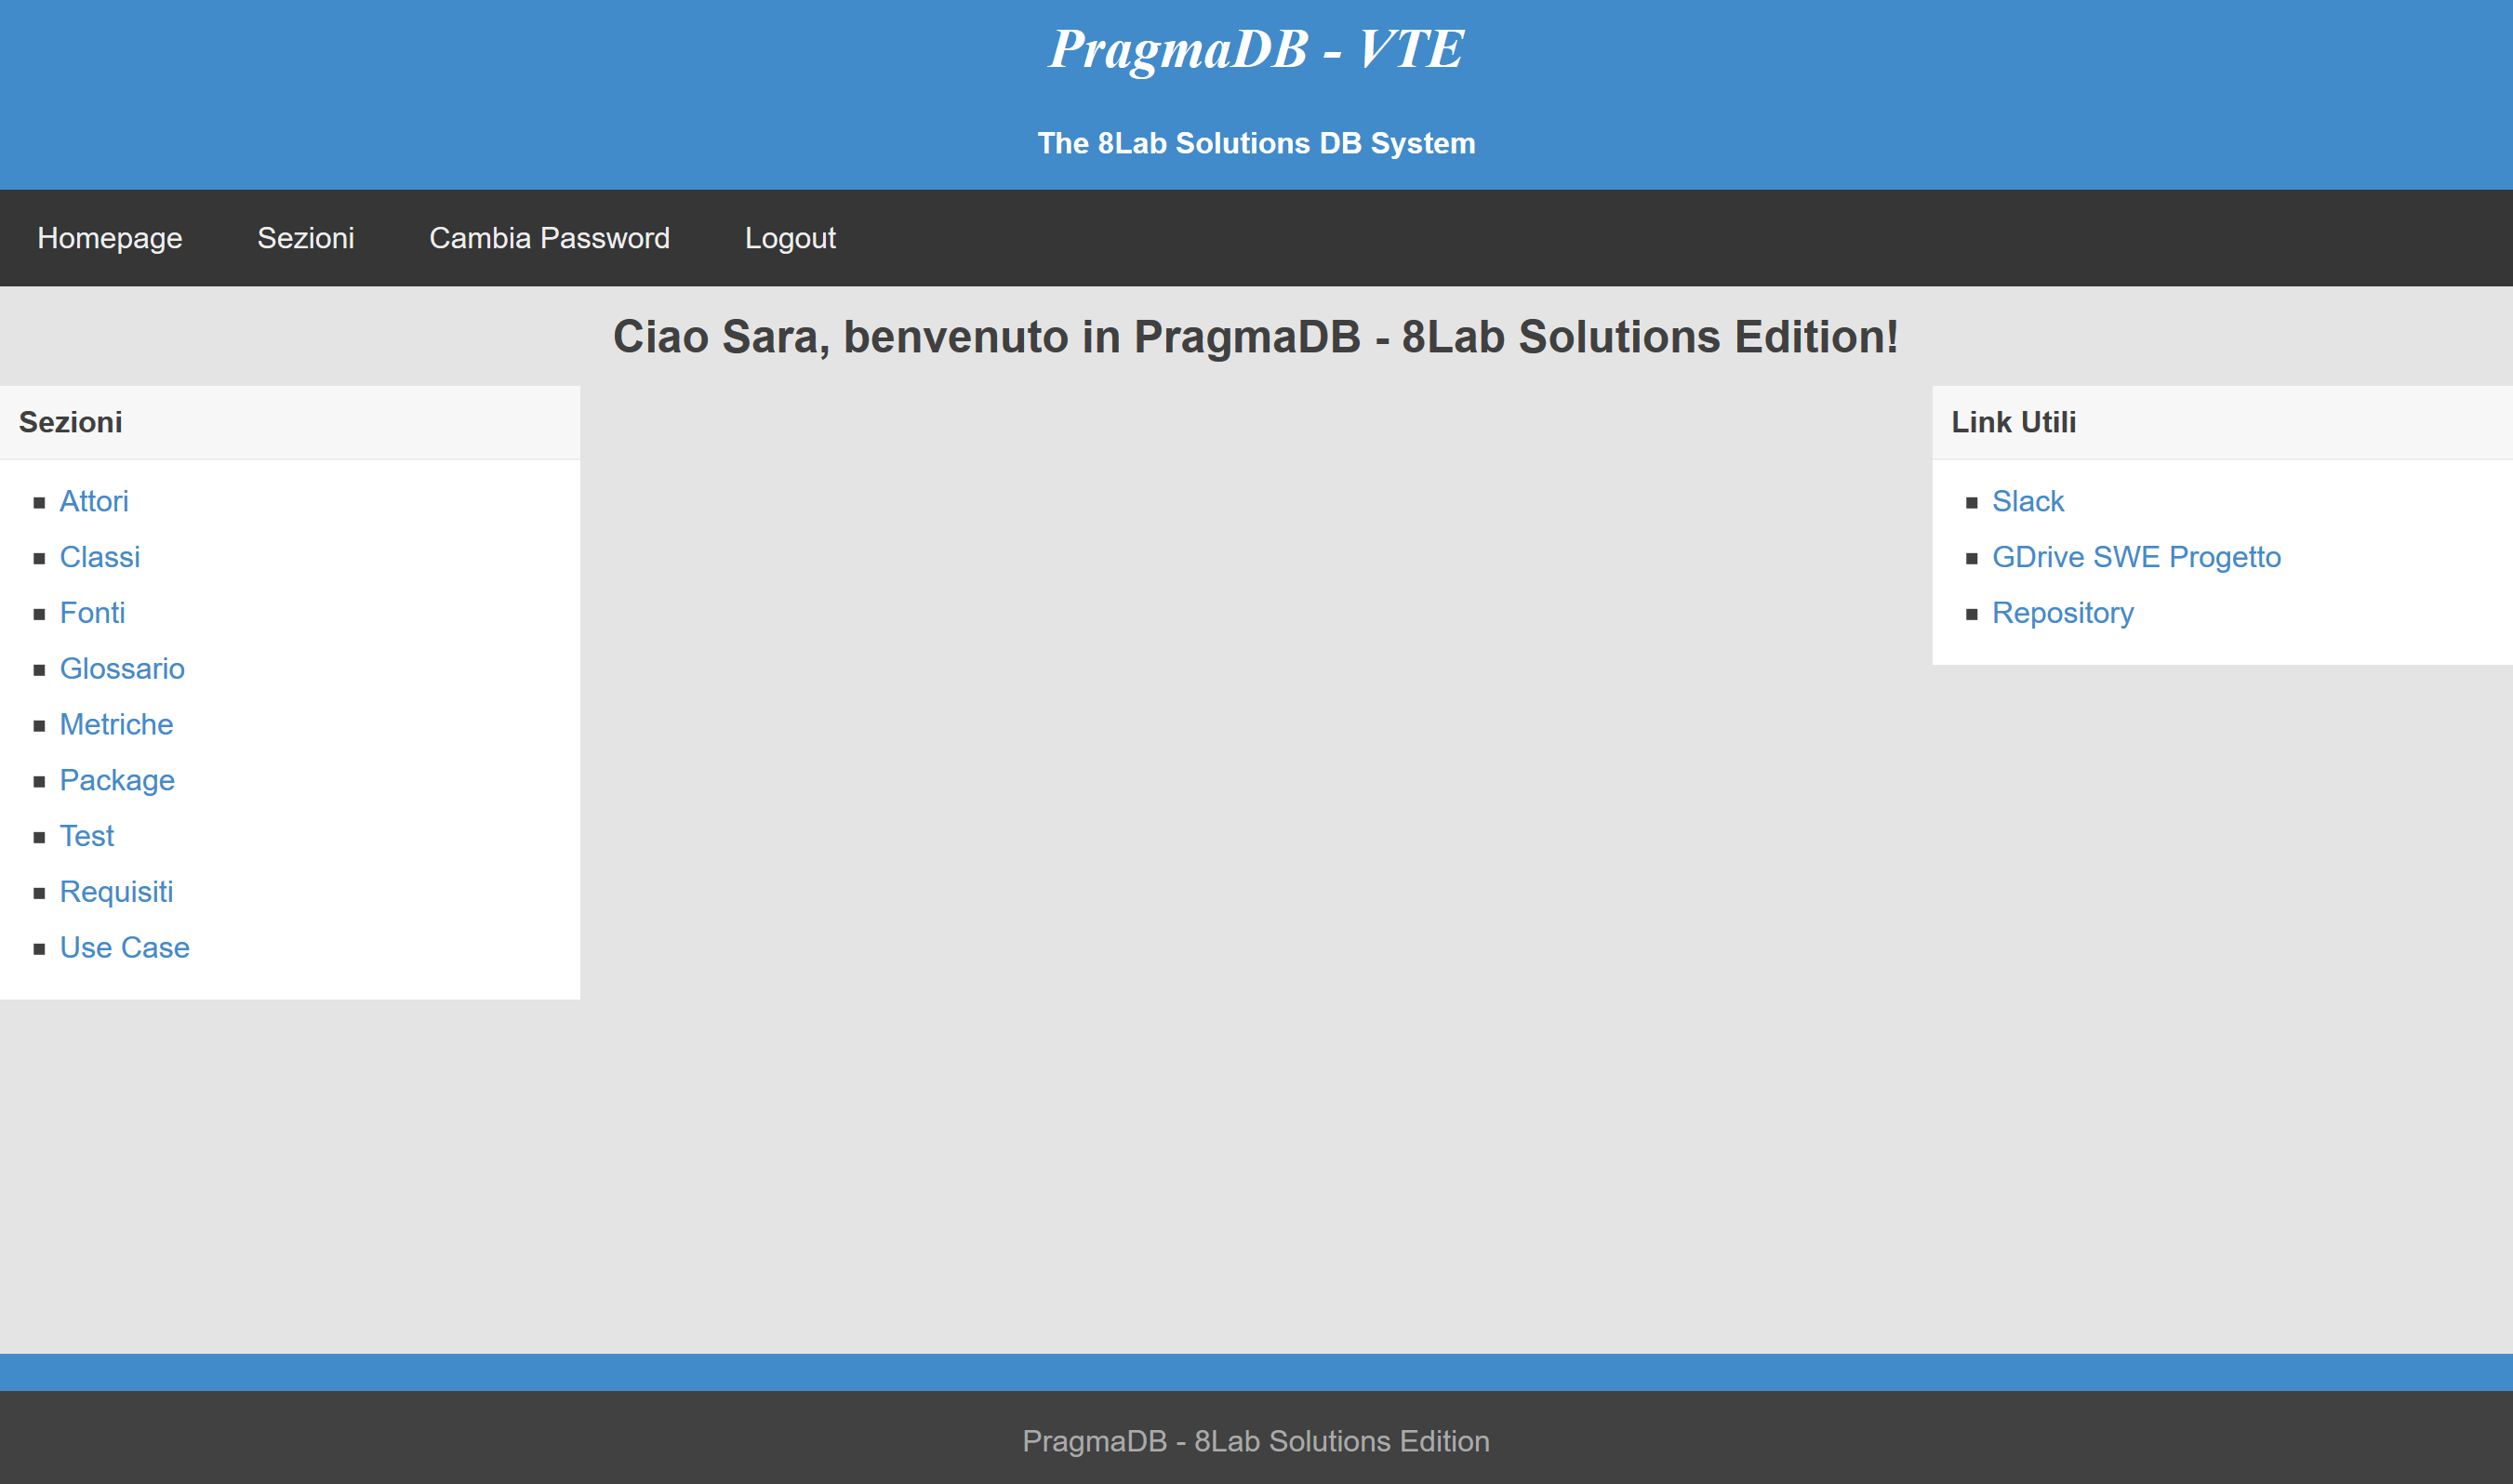
\includegraphics[width=0.99\linewidth]{res/images/HomepagePragmaDB.png}
		\caption{Homepage PragmaDB di un utente autenticato}
	\end{figure}
		
\paragraph{Draw.io} \mbox{}\\ \mbox{}\\
Per la produzione di diagrammi UML\glosp viene utilizzato Draw.io in quanto 
offre molte agevolazioni per la produzione veloce dei diagrammi e risulta 
semplice da usare. \newline
\centerline{\url{https://www.draw.io/}}
	\begin{figure}[H]
		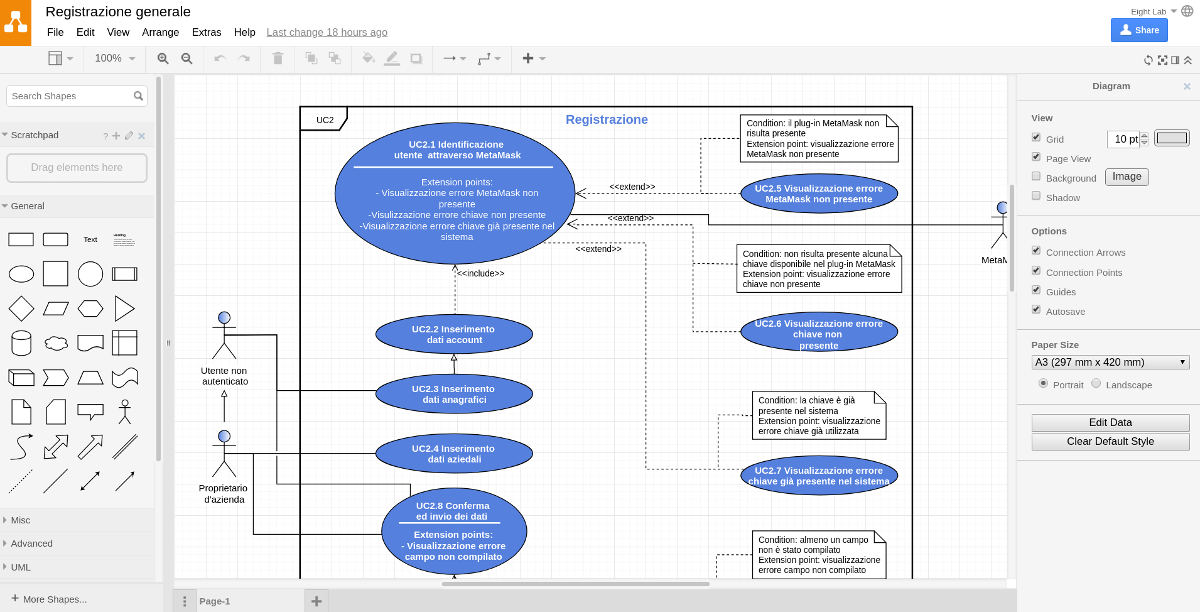
\includegraphics[width=0.99\linewidth]{res/images/drawio.jpg}
		\caption{Software per la creazione di diagrammi online}
	\end{figure} 
		
\paragraph{Visual Studio Code} \mbox{}\\ \mbox{}\\
Visual Studio Code viene utilizzato per la codifica in Solidity, Java e JavaScript. Questo 
IDE offre piena compatibilità con Linux, Windows, macOS, oltre ad essere un 
potente editor con molte funzionalità integrate. \newline
\centerline{\url{https://code.visualstudio.com/}}
	\begin{comment}
		\begin{figure}[H]
			\includegraphics[width=0.99\linewidth]{res/images/""}
			\caption{Software per la codifica}
		\end{figure} 
	\end{comment}
	
\paragraph{Truffle} \mbox{}\\ \mbox{}\\
Per lo sviluppo, test e gestione di smart contracts\glo, permette la scrittura automatizzata di test in JavaScript e Solidity\glo.\newline
\centerline{\url{https://truffleframework.com/truffle}}

\paragraph{React} \mbox{}\\ \mbox{}\\ 
Per la realizzazione dell'interfaccia utente a livello di applicazione web.\newline
\centerline{\url{https://reactjs.org/}}

\paragraph{Solidity} \mbox{}\\ \mbox{}\\ 
Per lo sviluppo di smart contracts\glo, tale linguaggio viene impiegato in Visual Studio Code.\newline
\centerline{\url{https://solidity.readthedocs.io/en/v0.5.3/}}

\paragraph{MetaMask} \mbox{}\\ \mbox{}\\ 
Utilizzato per effettuare transazioni sicure sulla rete Ethereum\glosp senza ospitare un nodo della rete e per eseguire ÐApps\glo. \newline
\centerline{\url{https://metamask.io/}}

\paragraph{Ganache} \mbox{}\\ \mbox{}\\
Impiegato per simulare una blockchain\glosp Ethereum\glosp locale.\\
\centerline{\url{https://truffleframework.com/ganache}}

\paragraph{Sass} \mbox{}\\ \mbox{}\\
Utilizzato per generare file CSS ottimizzati.\\
\centerline{\url{https://sass-lang.com/}}

\paragraph{Web3} \mbox{}\\ \mbox{}\\
Utilizzato per fare interagire il livello di back end\glosp con quello di front end\glo. \\
\centerline{\url{https://web3js.readthedocs.io/en/1.0/}}

\paragraph{Redux} \mbox{}\\ \mbox{}\\
Utilizzato per mantenere lo stato dell'applicazione.\\
\centerline{\url{https://redux.js.org/}}

\paragraph{Travis} \mbox{}\\ \mbox{}\\
Impiegato per garantire la continuous integration.\\
\centerline{\url{https://travis-ci.org/}}

\paragraph{Surge.sh} \mbox{}\\ \mbox{}\\
Utilizzato per favorire l'accessibilità del sito a livello globale, ovvero occupa la posizione di host dell'applicazione.\\
\centerline{\url{https://surge.sh/}}

\paragraph{Node.js} \mbox{}\\ \mbox{}\\
Utilizzato per creare applicazioni di rete scalabili non solo lato client ma anche lato server.\\
\centerline{\url{https://nodejs.org/it/about/}}

\paragraph{NPM} \mbox{}\\ \mbox{}\\
Utilizzato per poter installare i pacchetti necessari allo sviluppo dell'applicativo, quali React\glo, Redux\glo, Truffle\glo, Ganache CLI\glosp e Web3\glo. \\
\centerline{\url{https://www.npmjs.com/}}

\subsection{Procedure}
\subsubsection{Draw.io} 
\paragraph{Creazione dei diagrammi UML} \mbox{}\\ \mbox{}\\
Per la creazione dei diagrammi UML\glo{} è necessario accedere a Google Drive 
con le credenziali del gruppo, entrare nella cartella \texttt{Analisi dei requisiti} e 
successivamente nella cartella \texttt{UML Draw.io}. Un diagramma UML deve essere creato
rispettando il seguente ordine:
	\begin{itemize}
		\item nel menù \texttt{New}, scegliere \texttt{More} e quindi fare
			click \texttt{draw.io Diagrams};
		\item realizzare il diagramma con le convenzioni descritte nell'apposito
			paragrafo della sezione \ref{sec:UML}; 
		\item nel menù \texttt{File}, scegliere \texttt{Export as..} e selezionare \texttt{PNG};
		\item inserire un nome esplicativo (per es: UC14) e cliccare sull'icona di
			Google Drive;
		\item alla richiesta di selezionare in quale cartella salvare il diagramma 
			in formato PNG selezionare \texttt{No, pic folder..} e assicurarsi di salvare 
			nella cartella apposita denominata \texttt{png} (il percorso è 
			\texttt{Analisi dei requisiti > UML Draw.io > png}).
	\end{itemize}
Nella cartella \texttt{UML Draw.io} sono presente sia i file .io sia la cartella \texttt{png}
con gli stessi file in formato .png. Questa scelta permette di portare rapidamente 
delle modifiche ai diagrammi precedentemente disegnati. Inoltre, qualora venga 
effettuata una modifica, l'autore di tale modifica ha il compito di sostituire
il file .png aggiornato con quello precedente. 

\subsubsection{PragmaDB} 
Per eseguire le seguenti operazioni è necessario eseguire la login al sito \\
\centerline{\url{http://ec2-52-47-35-145.eu-west-3.compute.amazonaws.com/PragmaDB/PHP/}}
in cui ogni membro del gruppo deve inserire username e password.

\paragraph{Aggiungere un attore} \mbox{}\\ \mbox{}\\
Dopo aver eseguito l'autenticazione:
\begin{itemize}
	\item selezionare \texttt{Attori} nel pannello posto a sinistra;
	\item selezionare \texttt{Inserisci Attore} nel panello posto a destra;
	\item compilare il form per l'inserimento di un nuovo attore, inserendo 
		il nome e la descrizione relativi ad esso;
	\item cliccare sul tasto \texttt{Conferma} per aggiungere il nuovo attore 
		creato oppure \texttt{Cancella} per tornare indietro.	
\end{itemize}

\paragraph{Modificare un attore} \mbox{}\\ \mbox{}\\
Dopo aver eseguito l'autenticazione:
\begin{itemize}
	\item selezionare \texttt{Attori} nel pannello posto a sinistra;
	\item selezionare \texttt{Modifica} dalla riga della tabella dell'attore
		che si vuole modificare;
	\item modificare i campi del form dell'attore selezionato;
	\item cliccare sul tasto \texttt{Modifica} per salvare le modifiche effettuate
		oppure \texttt{Cancella} per tornare indietro.	
\end{itemize}

\paragraph{Eliminare un attore} \mbox{}\\ \mbox{}\\
Dopo aver eseguito l'autenticazione:
\begin{itemize}
	\item selezionare \texttt{Attori} nel pannello posto a sinistra;
	\item selezionare \texttt{Elimina} dalla riga della tabella dell'attore
		che si vuole eliminare;
	\item cliccare sul tasto \texttt{Elimina} per confermare la rimozione
		oppure \texttt{Cancella} per tornare indietro.	
\end{itemize}

\paragraph{Aggiungere una classe} \mbox{}\\ \mbox{}\\
Dopo aver eseguito l'autenticazione:
\begin{itemize}
	\item selezionare \texttt{Classi} nel pannello posto a sinistra;
	\item selezionare \texttt{Inserisci Classe} nel panello posto a destra;
	\item compilare il form per l'inserimento di una nuova classe;
	\item cliccare sul tasto \texttt{Inserisci} per aggiungere la nuova classe 
		creata oppure \texttt{Cancella} per tornare indietro.	
\end{itemize}

\paragraph{Modificare una classe} \mbox{}\\ \mbox{}\\
Dopo aver eseguito l'autenticazione:
\begin{itemize}
	\item selezionare \texttt{Classi} nel pannello posto a sinistra;
	\item selezionare \texttt{Modifica} dalla riga della tabella della classe
		che si vuole modificare;
	\item modificare i campi del form della classe selezionata;
	\item cliccare sul tasto \texttt{Modifica} per salvare le modifiche effettuate
		oppure \texttt{Cancella} per tornare indietro.
\end{itemize}

\paragraph{Eliminare una classe} \mbox{}\\ \mbox{}\\
Dopo aver eseguito l'autenticazione:
\begin{itemize}
	\item selezionare \texttt{Classi} nel pannello posto a sinistra;
	\item selezionare \texttt{Eliminare} dalla riga della tabella della classe
		che si vuole eliminare;
	\item cliccare sul tasto \texttt{Elimina} per confermare la rimozione della classe
		oppure \texttt{Annulla} per tornare indietro.
\end{itemize}

\paragraph{Aggiungere un attributo alla classe} \mbox{}\\ \mbox{}\\
Dopo aver eseguito l'autenticazione:
\begin{itemize}
	\item selezionare \texttt{Classi} nel pannello posto a sinistra;
	\item selezionare \texttt{Attributi} dalla riga della tabella della classe
		a cui si vuole aggiungere un attributo;
	\item selezionare \texttt{Inserisci Attributo} dal pannello posto a destra;
	\item compilare il form per l'inserimento di un nuovo attributo;
	\item cliccare sul tasto \texttt{Inserisci} per aggiungere il nuovo attributo 
		creato oppure \texttt{Cancella} per tornare indietro.	
\end{itemize}

\paragraph{Modificare un attributo alla classe} \mbox{}\\ \mbox{}\\
Dopo aver eseguito l'autenticazione:
\begin{itemize}
	\item selezionare \texttt{Classi} nel pannello posto a sinistra;
	\item selezionare \texttt{Attributi} dalla riga della tabella della classe
		a cui si vuole modificare un attributo;\
	\item selezionare \texttt{Modifica} dalla riga della tabella dell'attributo
		che si vuole modificare;
	\item modificare i campi del form dell'attributo selezionato;
	\item cliccare sul tasto \texttt{Modifica} per salvare le modifiche effettuate
		oppure \texttt{Cancella} per tornare indietro.
\end{itemize}

\paragraph{Eliminare un attributo alla classe} \mbox{}\\ \mbox{}\\
Dopo aver eseguito l'autenticazione:
\begin{itemize}
	\item selezionare \texttt{Classi} nel pannello posto a sinistra;
	\item selezionare \texttt{Attributi} dalla riga della tabella della classe
		a cui si vuole eliminare un attributo;\
	\item selezionare \texttt{Eliminare} dalla riga della tabella dell'attributo 
		che si vuole eliminare;
	\item cliccare sul tasto \texttt{Elimina} per confermare la rimozione dell'attributo
		oppure \texttt{Annulla} per tornare indietro.
\end{itemize}

\paragraph{Aggiungere un metodo alla classe} \mbox{}\\ \mbox{}\\
Dopo aver eseguito l'autenticazione:
\begin{itemize}
	\item selezionare \texttt{Classi} nel pannello posto a sinistra;
	\item selezionare \texttt{Metodi} dalla riga della tabella della classe
		a cui si vuole aggiungere un metodo;
	\item selezionare \texttt{Inserisci Metodo} dal pannello posto a destra;
	\item compilare il form per l'inserimento di un nuovo metodo;
	\item cliccare sul tasto \texttt{Inserisci} per aggiungere il nuovo metodo 
		creato oppure \texttt{Cancella} per tornare indietro.	
\end{itemize}

\paragraph{Modificare un metodo alla classe} \mbox{}\\ \mbox{}\\
Dopo aver eseguito l'autenticazione:
\begin{itemize}
	\item selezionare \texttt{Classi} nel pannello posto a sinistra;
	\item selezionare \texttt{Metodi} dalla riga della tabella della classe
		a cui si vuole modificare un metodo;
	\item selezionare \texttt{Inserisci Metodo} dal pannello posto a destra;
	\item modificare i campi del form del metodo selezionato;
	\item cliccare sul tasto \texttt{Modifica} per salvare le modifiche effettuate
		oppure \texttt{Cancella} per tornare indietro.	
\end{itemize}

\paragraph{Eliminare un metodo alla classe} \mbox{}\\ \mbox{}\\
Dopo aver eseguito l'autenticazione:
\begin{itemize}
	\item selezionare \texttt{Classi} nel pannello posto a sinistra;
	\item selezionare \texttt{Attributi} dalla riga della tabella della classe
		a cui si vuole eliminare un metodo;\
	\item selezionare \texttt{Eliminare} dalla riga della tabella del metodo
		che si vuole eliminare;
	\item cliccare sul tasto \texttt{Elimina} per confermare la rimozione del metodo
		oppure \texttt{Annulla} per tornare indietro.
\end{itemize}

\paragraph{Aggiungere un requisito alla classe} \mbox{}\\ \mbox{}\\
Dopo aver eseguito l'autenticazione:
\begin{itemize}
	\item selezionare \texttt{Classi} nel pannello posto a sinistra;
	\item selezionare \texttt{Requisiti} dalla riga della tabella della classe
		a cui si vuole aggiungere un requisito;
	\item selezionare \texttt{Inserisci Requisito} dal pannello posto a destra;
	\item compilare il form per l'inserimento di un nuovo metodo;
	\item cliccare sul tasto \texttt{Inserisci} per aggiungere il nuovo metodo 
		creato oppure \texttt{Cancella} per tornare indietro.	
\end{itemize}

\paragraph{Modificare un requisito alla classe} \mbox{}\\ \mbox{}\\
Dopo aver eseguito l'autenticazione:
\begin{itemize}
	\item selezionare \texttt{Classi} nel pannello posto a sinistra;
	\item selezionare \texttt{Requisiti} dalla riga della tabella della classe
		a cui si vuole modificare un requisito;
	\item selezionare \texttt{Inserisci Requisito} dal pannello posto a destra;
	\item modificare i campi del form del requisito selezionato;
	\item cliccare sul tasto \texttt{Modifica} per salvare le modifiche effettuate
		oppure \texttt{Cancella} per tornare indietro.
\end{itemize}

\paragraph{Eliminare un requisito alla classe} \mbox{}\\ \mbox{}\\
Dopo aver eseguito l'autenticazione:
\begin{itemize}
	\item selezionare \texttt{Classi} nel pannello posto a sinistra;
	\item selezionare \texttt{Requisiti} dalla riga della tabella della classe
		a cui si vuole eliminare un requisito;\
	\item selezionare \texttt{Eliminare} dalla riga della tabella del requisito
		che si vuole eliminare;
	\item cliccare sul tasto \texttt{Elimina} per confermare la rimozione del requisito
		oppure \texttt{Annulla} per tornare indietro.
\end{itemize}

\paragraph{Aggiungere una fonte} \mbox{}\\ \mbox{}\\
Dopo aver eseguito l'autenticazione:
\begin{itemize}
	\item selezionare \texttt{Fonti} nel pannello posto a sinistra;
	\item selezionare \texttt{Inserisci Fonte} dal pannello posto a destra;
	\item compilare il form per l'inserimento di una nuova fonte;
	\item cliccare sul tasto \texttt{Inserisci} per aggiungere la nuova fonte 
		creata oppure \texttt{Cancella} per tornare indietro.	
\end{itemize}

\paragraph{Modificare una fonte} \mbox{}\\ \mbox{}\\
Dopo aver eseguito l'autenticazione:
\begin{itemize}
	\item selezionare \texttt{Fonti} nel pannello posto a sinistra;
	\item selezionare \texttt{Modifica} dalla riga della tabella della fonte
		che si vuole modificare;
	\item modificare i campi del form della fonte selezionata;
	\item cliccare sul tasto \texttt{Modifica} per salvare le modifiche effettuate
		oppure \texttt{Cancella} per tornare indietro.
\end{itemize}

\paragraph{Eliminare una fonte} \mbox{}\\ \mbox{}\\\\
Dopo aver eseguito l'autenticazione:
\begin{itemize}
	\item selezionare \texttt{Fonti} nel pannello posto a sinistra;
	\item selezionare \texttt{Elimina} dalla riga della tabella della fonte 
		che si vuole eliminare;\
	\item cliccare sul tasto \texttt{Elimina} per confermare la rimozione della fonte
		oppure \texttt{Annulla} per tornare indietro.
\end{itemize}

\paragraph{Aggiungere un package} \mbox{}\\ \mbox{}\\
Dopo aver eseguito l'autenticazione:
\begin{itemize}
	\item selezionare \texttt{Package} nel pannello posto a sinistra;
	\item selezionare \texttt{Inserisci Package} dal pannello posto a destra;
	\item compilare il form per l'inserimento di un nuovo package;
	\item cliccare sul tasto \texttt{Inserisci} per aggiungere il nuovo package
		creato oppure \texttt{Cancella} per tornare indietro.	
\end{itemize}

\paragraph{Modificare un package} \mbox{}\\ \mbox{}\\
Dopo aver eseguito l'autenticazione:
\begin{itemize}
	\item selezionare \texttt{Package} nel pannello posto a sinistra;
	\item selezionare \texttt{Modifica} dalla riga della tabella del package
		che si vuole modificare;
	\item modificare i campi del form del package selezionato;
	\item cliccare sul tasto \texttt{Modifica} per salvare le modifiche effettuate
		oppure \texttt{Cancella} per tornare indietro.
\end{itemize}

\paragraph{Eliminare un package} \mbox{}\\ \mbox{}\\
Dopo aver eseguito l'autenticazione:
\begin{itemize}
	\item selezionare \texttt{Package} nel pannello posto a sinistra;
	\item selezionare \texttt{Elimina} dalla riga della tabella del package 
		che si vuole eliminare;\
	\item cliccare sul tasto \texttt{Elimina} per confermare la rimozione del package
		oppure \texttt{Annulla} per tornare indietro.
\end{itemize}

\paragraph{Aggiungere un test} \mbox{}\\ \mbox{}\\
Dopo aver eseguito l'autenticazione:
\begin{itemize}
	\item selezionare \texttt{Test} nel pannello posto a sinistra;
	\item selezionare \texttt{Inserisci Test} dal pannello posto a destra;
	\item compilare il form per l'inserimento di un nuovo test;
	\item cliccare sul tasto \texttt{Inserisci} per aggiungere il nuovo test
		creato oppure \texttt{Cancella} per tornare indietro.	
\end{itemize}

\paragraph{Modificare un test} \mbox{}\\ \mbox{}\\
Dopo aver eseguito l'autenticazione:
\begin{itemize}
	\item selezionare \texttt{Test} nel pannello posto a sinistra;
	\item selezionare \texttt{Modifica} dalla riga della tabella del test
		che si vuole modificare;
	\item modificare i campi del form del test selezionato;
	\item cliccare sul tasto \texttt{Modifica} per salvare le modifiche effettuate
		oppure \texttt{Cancella} per tornare indietro.
\end{itemize}

\paragraph{Eliminare un test} \mbox{}\\ \mbox{}\\
Dopo aver eseguito l'autenticazione:
\begin{itemize}
	\item selezionare \texttt{Test} nel pannello posto a sinistra;
	\item selezionare \texttt{Elimina} dalla riga della tabella del test
		che si vuole eliminare;\
	\item cliccare sul tasto \texttt{Elimina} per confermare la rimozione del test
		oppure \texttt{Annulla} per tornare indietro.
\end{itemize}		

\paragraph{Aggiungere un requisito} \mbox{}\\ \mbox{}\\
Dopo aver eseguito l'autenticazione:
\begin{itemize}
	\item selezionare \texttt{Requisiti} nel pannello posto a sinistra;
	\item selezionare \texttt{Inserisci Requisiti} dal pannello posto a destra;
	\item compilare il form per l'inserimento di un nuovo requisito;
	\item cliccare sul tasto \texttt{Inserisci} per aggiungere il nuovo requisito
		creato oppure \texttt{Cancella} per tornare indietro.	
\end{itemize}

\paragraph{Modificare un requisito} \mbox{}\\ \mbox{}\\
Dopo aver eseguito l'autenticazione:
\begin{itemize}
	\item selezionare \texttt{Requisiti} nel pannello posto a sinistra;
	\item selezionare \texttt{Modifica} dalla riga della tabella del requisito
		che si vuole modificare;
	\item modificare i campi del form del requisito selezionato;
	\item cliccare sul tasto \texttt{Modifica} per salvare le modifiche effettuate
		oppure \texttt{Cancella} per tornare indietro.
\end{itemize}

\paragraph{Eliminare un requisito} \mbox{}\\ \mbox{}\\
Dopo aver eseguito l'autenticazione:
\begin{itemize}
	\item selezionare \texttt{Requisiti} nel pannello posto a sinistra;
	\item selezionare \texttt{Elimina} dalla riga della tabella del requisito 
		che si vuole eliminare;\
	\item cliccare sul tasto \texttt{Elimina} per confermare la rimozione del requisito
		oppure \texttt{Annulla} per tornare indietro.
\end{itemize}

\paragraph{Aggiungere un use case} \mbox{}\\ \mbox{}\\
Dopo aver eseguito l'autenticazione:
\begin{itemize}
	\item selezionare \texttt{Use Case} nel pannello posto a sinistra;
	\item selezionare \texttt{Inserisci Use Case} dal pannello posto a destra;
	\item compilare il form per l'inserimento di un nuovo use case;
	\item cliccare sul tasto \texttt{Inserisci} per aggiungere il nuovo use case
		creato oppure \texttt{Cancella} per tornare indietro.	
\end{itemize}

\paragraph{Modificare un use case} \mbox{}\\ \mbox{}\\
Dopo aver eseguito l'autenticazione:
\begin{itemize}
	\item selezionare \texttt{Use Case} nel pannello posto a sinistra;
	\item selezionare \texttt{Modifica} dalla riga della tabella del use case
		che si vuole modificare;
	\item modificare i campi del form del use case selezionato;
	\item cliccare sul tasto \texttt{Modifica} per salvare le modifiche effettuate
		oppure \texttt{Cancella} per tornare indietro.
\end{itemize}

\paragraph{Eliminare un use case} \mbox{}\\ \mbox{}\\
Dopo aver eseguito l'autenticazione:
\begin{itemize}
	\item selezionare \texttt{Use Case} nel pannello posto a sinistra;
	\item selezionare \texttt{Elimina} dalla riga della tabella del use case 
		che si vuole eliminare;\
	\item cliccare sul tasto \texttt{Elimina} per confermare la rimozione del use case
		oppure \texttt{Annulla} per tornare indietro.
\end{itemize}


	\pagebreak
	
	\section{Processi di supporto}
\subsection{Documentazione}
	\subsubsection{Scopo}
	Ogni processo e attività significativi volti allo sviluppo del progetto sono documentati. Lo scopo di questa sezione è definire gli standard che riguardano i documenti prodotti durante il ciclo di vita del software.
	I documenti sono consultabili nelle apposite sezioni della repository\glo:\\
	\centerline{\url{https://github.com/8LabSolutions/Soldino}} 		
	\subsubsection{Aspettative}
	Le aspettative su questo processo riguardano:
	\begin{itemize}
		\item un'idea precisa relativa alla struttura della documentazione che deve essere prodotta durante il ciclo di vita del software;
		\item l'individuazione di una serie di norme per la stesura di documenti coerenti e validi.
	\end{itemize}
	\subsubsection{Descrizione}
	Questo capitolo contiene le decisioni e le norme che sono state scelte per la
	stesura, verifica e approvazione della documentazione ufficiale.  Tali norme  sono  tassative  per  tutti  i  documenti  formali.
	\subsubsection{Ciclo di vita del documento}
	Ogni documento segue le fasi del seguente ciclo di vita:
	\begin{itemize}
		\item \textbf{Creazione del documento}: il documento viene creato, in conformità alle norme e adeguandosi a documenti precedenti dello stesso tipo.
		Viene usato un template reperibile dalla cartella "latex" della repository\glosp remota;
		\item \textbf{Creazione della struttura}: viene creato un registro delle modifiche, un indice che traccia gli argomenti trattati nel documento, e a seconda delle necessità, un indice relativo alle figure e uno relativo alle tabelle presenti nel documento;
		\item \textbf{Realizzazione}: il documento viene scritto progressivamente in modo incrementale;
		\item \textbf{In revisione}: ogni voce del documento è prodotta interamente, ma è soggetta a verifiche per correggere, ampliare, semplificare quanto presente. La verifica di un frammento è svolta da almeno una persona, diversa da quella che ha scritto quel frammento;
		\item \textbf{Approvato}: il responsabile di progetto sancisce che il documento è stato completato, ed è quindi pronto per il rilascio.
	\end{itemize}

	\subsubsection{Template}
	Il gruppo ha creato un template \LaTeX{} per uniformare velocemente la 
	struttura grafica e lo stile di formattazione dei documenti, in modo che i 
	membri del team possano concentrarsi maggiormente, nella stesura del 
	contenuto degli stessi. Lo scopo dei template è di permettere, a colui che 
	redige il documento, di adottare automaticamente le conformità previste 
	dalle \textit{Norme di Progetto}. Permette inoltre di agevolare la 
	procedura di adeguamento alle nuove norme per la redazione, nel caso esse 
	cambiassero.
	\subsubsection{Struttura dei documenti}
	Un file "main.tex" (il cui termine "main" verrà sostituito dal nome del documento) raccoglie tramite comandi di input le sezioni di cui è composto il documento. Tra i file in input ci sono:
	\begin{itemize}
		\item "package.tex", che contiene i pacchetti necessari alla compilazione;
		\item "config.tex", contenente comandi \LaTeX{} creati dal team.
	\end{itemize}
		\paragraph{Prima pagina} \mbox{}\\ \mbox{}\\
		Il frontespizio è la prima pagina del documento ed è così strutturata:
		\begin{itemize}
			\item \textbf{Logo del gruppo}: logo di \textit{8Lab Solutions} visibile come primo elemento centrato orizzontalmente in alto;
			\item \textbf{Gruppo e progetto}: nome del gruppo e del progetto \textit{Soldino}, visibile centralmente subito sotto il logo;
			\item \textbf{Titolo}: nome del documento, posizionato centralmente in grassetto;
			\item \textbf{Tabella}: presente sotto il titolo del documento, centrale e contenente le seguenti informazioni:
			\begin{itemize}
				\item \textbf{Versione}: versione del documento;
				\item \textbf{Approvazione}: nome e cognome dei membri del gruppo incaricati dell'approvazione del documento;
				\item \textbf{Redazione}: nome e cognome dei membri del gruppo incaricati della redazione del documento;
				\item \textbf{Verifica}: nome e cognome dei membri del gruppo incaricati della verifica del documento;
				\item \textbf{Stato}: stadio corrente del ciclo di vita del documento;
				\item \textbf{Uso}: tipo d'uso che può essere "interno" o "esterno";
				\item \textbf{Destinato a}: destinatari del documento.
			\end{itemize}
			\item \textbf{Descrizione}: descrizione sintetica relativa al documento, centrale, posta sotto la tabella descrittiva;
			\item \textbf{Recapito}: indirizzo di posta elettronica del gruppo, posizionato centralmente in fondo alla pagina.
		\end{itemize}
		\paragraph{Registro modifiche} \mbox{}\\ \mbox{}\\
		Ogni documento dispone di un changelog\glo: una tabella posta a seguito della prima pagina che contiene le modifiche apportate al documento. Nel changelog\glosp sono indicati:
		\begin{itemize}
			\item versione del documento dopo la modifica;
			\item data della modifica;
			\item nominativo di chi ha modificato;
			\item ruolo di chi ha modificato;
			\item descrizione sintetica della modifica.
		\end{itemize}
		\paragraph{Indice} \mbox{}\\ \mbox{}\\
		Gli indici hanno lo scopo di riepilogare e dare una visione macroscopica della struttura del documento, mostrando le parti gerarchiche di cui è composto.\newline 
		Ogni documento è corredato dall'indice dei contenuti, posizionato dopo il changelog\glo{}. Se sono presenti tabelle o immagini all'interno del documento, l'indice dei contenuti è seguito prima dalla lista delle figure, poi dalla lista delle tabelle.
		\paragraph{Contenuto principale} \mbox{}\\ \mbox{}\\
		La struttura delle pagine di contenuto è così strutturata:
		\begin{itemize}
			\item in alto a sinistra è presente il logo del gruppo;
			\item in alto a destra è riportato il nome del documento;
			\item una riga divide l'intestazione dal contenuto;
			\item il contenuto della pagina è posto tra l'intestazione e il piè di pagina;
			\item una riga divide il contenuto dal piè pagina;
			\item in basso a destra è posto il numero della pagina corrente.
		\end{itemize}
		\paragraph{Verbali} \mbox{}\\ \mbox{}\\
		I verbali vengono prodotti dal soggetto incaricato alla loro stesura in occasione di incontri tra i membri del team con o senza la presenza di esterni. Per i verbali è prevista un'unica stesura. Tale	scelta è motivata dal fatto che apportare modifiche implica una modifica delle decisioni prese in modo retroattivo.
		I verbali seguono la struttura degli altri documenti, ma il corpo del verbale è suddiviso in introduzione e contenuto.
		L'introduzione contiene:
		\begin{itemize}
			\item \textbf{Luogo}: luogo di svolgimento dell'incontro;
			\item \textbf{Data}: data dell'incontro(in formato YYYY-MM-DD);
			\item \textbf{Ora di inizio}: l'orario di inizio dell'incontro;
			\item \textbf{Ora di fine}: l'orario di fine dell'incontro;
			\item \textbf{Segretario}: membro del gruppo che redige il documento;
			\item \textbf{Partecipanti}: l'elenco dei membri del gruppo che erano presenti all'incontro e, se presenti, i nominativi di persone esterne al gruppo che hanno partecipato. Un esempio, sono i nomi dei componenti di \textit{Red Babel}, a fianco al quale deve essere indicato "(proponente)";
			\item \textbf{Argomenti affrontati}: ciò di cui si è discusso durante l'incontro in forma riassuntiva e facendo risaltare gli argomenti principali.
		\end{itemize}
	Il contenuto è composto da:
	\begin{itemize}
		\item una descrizione più approfondita in merito agli argomenti trattati durante l'incontro;
		\item un riepilogo dei tracciamenti in forma tabellare che elenca le decisioni emerse: assegna ad ognuna di loro un codice e le descrive. Sarà ripresa successivamente.
	\end{itemize}
		Ogni \textit{Verbale} dovrà essere denominato secondo il seguente formato: \newline \newline
		\centerline{\textbf{verbale\_tipologia\_YYYY-MM-DD}} \newline \newline
		dove per "tipologia" si intende il tipo di verbale:
		\begin{itemize}
			\item \textbf{interno}: concentrato sul riassunto dell'incontro dei membri del team;
			\item \textbf{esterno}: concentrato sulla trattazione di argomenti con partecipanti esterni al gruppo, in particolare domande e risposte riguardanti il progetto in sé.
		\end{itemize}
		La sezione "Riepilogo tracciamenti" avrà la funzione di tenere traccia delle decisioni emerse da ogni incontro, sotto forma di tabella riassuntiva a fine di ogni verbale. Il formalismo utilizzato dalla tabella dovrà essere il seguente: \newline \newline
		\centerline{\textbf{Tipologia\_X.Y}} \newline \newline
		Dove:
		\begin{itemize}
			\item per "Tipologia" basterà indicare l'iniziale della tipologia del verbale (VI = Interno, VE = Esterno);
			\item "X.Y": X si riferisce al numero dell'incontro mentre per Y si intende il numero progressivo della decisione presa dal gruppo (partendo da 1).
		\end{itemize}	
		\paragraph{Note a piè di pagina} \mbox{}\\ \mbox{}\\
		In caso di presenza di note da esplicare, esse vanno indicate nella pagina corrente, in basso a sinistra. Ogni nota deve riportare un numero e una descrizione.		
	\subsubsection{Norme tipografiche}
		\paragraph{Convenzioni sui nomi dei file} \mbox{}\\ \mbox{}\\
		I nomi di file (estensione esclusa) e cartelle utilizzano la convenzione "Snake case\glo" e alcune regole aggiuntive elencate di seguito:
		\begin{enumerate}
			\item i nomi dei file composti da più parole usano il carattere underscore come carattere separatore;
			\item i nomi sono scritti interamente in minuscolo;
			\item le preposizioni non si omettono.
		\end{enumerate}
		Alcuni esempi \textbf{corretti} sono:
		\begin{itemize}
			\item studio\_di\_fattibilità;
			\item analisi\_dei\_requisiti.
		\end{itemize}	 	
		Alcuni esempi \textbf{non corretti} sono: 
		\begin{itemize}
			\item Norme\_di\_progetto (usa maiuscole);
			\item norme-di-progetto (carattere separatore errato);
			\item norme\_progetto (omette "di").
		\end{itemize}
		\paragraph{Glossario}
		\begin{itemize}
			\item ogni termine del \textit{Glossario} è marcato con una \textbf{G} maiuscola a pedice in ogni sua occorrenza;
			\item se la voce è presente ripetutamente nello stesso paragrafo non è necessario marcarla in ogni sua occorrenza, ma è possibile indicare la \textbf{G} a pedice solo nella prima occorrenza;
			\item se nel \textit{Glossario} un termina presenta una descrizione che utilizza termini da glossario, è necessario trattare questi termini come tali, segnando la \textbf{G} a pedice e aggiungendoli al documento con la relativa descrizione;
			\item non vengono segnate con la \textbf{G} a pedice  le parole da glossario presenti nei titoli e nelle didascalie di immagini e tabelle.
		\end{itemize}			
		\paragraph{Stile del testo}
		\begin{itemize}
			\item \textbf{Grassetto}:
			viene applicato se necessario alle voci di un elenco puntato, a titoli o a termini di frasi su cui si vuol far ricadere l'attenzione del lettore;
			\item \textbf{Corsivo}: vengono scritti in corsivo il nome del progetto \textit{Soldino}, il nome del gruppo \textit{8Lab Solutions} ed il nome del gruppo dei proponenti, ovvero \textit{Red Babel}; %token\glosp coniato nella piattaforma,  \textit{Cubit};
			\item \textbf{Maiuscolo}: vengono scritti con sole lettere maiuscole tutti gli acronimi. Nel caso di nomi o titoli composti da più parole verrà indicato con la lettera maiuscola solamente la prima lettera della prima parola, lasciando in minuscolo il restante (esclusi nomi dei documenti che sono normati secondo quanto segue);
			\item \textbf{Nomi dei documenti}:
			\begin{itemize}
				\item ogni volta che si cita un documento, si deve indicare con la lettera maiuscola le iniziali dei nomi di cui è composto (\textit{e.g.} Analisi dei Requisiti), ma senza specificare la versione, riportando il tutto in corsivo;
				\item quando si fa riferimento al documento vero e proprio o a qualcosa in esso contenuto si segue la prima convenzione ma si aggiunge la versione del documento v*.0.0 (separata da uno spazio), anch'essa in corsivo;
				\item ogni volta che si utilizza il documento come titolo o in una voce di elenco seguita da una descrizione, si deve seguire la prima convenzione ma senza utilizzare il corsivo.
			\end{itemize}
		\end{itemize}
		\paragraph{Elenchi puntati} \mbox{}\\ \mbox{}\\
		Ogni voce di un elenco comincia per lettera \textbf{minuscola}, a patto che non subentrino altre norme, e termina per \textbf{";"}, eccetto l'ultima che termina per \textbf{"."}. I sottoelenchi innestati dentro una voce di elenco, rispettano le medesime regole, poiché la loro funzione è analoga.\newline
		Se le voci dell'elenco sono della forma \textit{termine - descrizione}, si pongono i termini in grassetto.
		\paragraph{Formati comuni} \mbox{}\\ \mbox{}\\
		In conformità allo standard ISO 8601, le date devono essere scritte secondo il formato: \newline \newline
		\centerline{YYYY-MM-DD}
		\begin{itemize}
			\item \textbf{YYYY}: rappresentazione dell'anno con quattro cifre;
			\item\textbf{MM}: rappresentazione del mese con due cifre;
			\item \textbf{DD}: rappresentazione del giorno con due cifre.			
		\end{itemize}
		\paragraph{Sigle} \mbox{}\\ \mbox{}\\
		Il progetto prevede la redazione di un insieme di documenti, suddivisi in interni e esterni. Essi sono elencati di seguito con le rispettive sigle.\newline
		I documenti esterni sono:	
		\begin{itemize}
			\item \textbf{Analisi dei Requisiti - AdR}: stabilisce le specifiche del software;
			\item \textbf{Manuale Utente - MU}: ad uso degli utenti del software;
			\item \textbf{Manuale Sviluppatore - MS}: per gli sviluppatori e manutentori del software;
			\item \textbf{Piano di Progetto - PdP}:  concerne la gestione del progetto, evidenziandone la fattibilità e le criticità; tratta di tempi, costi, obiettivi, rischi, vincoli;
			\item \textbf{Piano di Qualifica - PdQ}: : descrive la qualità del software e dei processi, e come la si intende raggiungere mediante l'uso di strumenti, metriche, verifiche e test.
		\end{itemize}
		I documenti interni sono:
		\begin{itemize}
			\item \textbf{Glossario - G}: raccoglie i termini di interesse per il team di sviluppo e dei quali è necessaria una descrizione che ne chiarisca il significato;
			\item \textbf{Norme di Progetto - NdP}: sono un riferimento normativo per lo svolgimento delle attività di progetto;
			\item \textbf{Studio di Fattibilità - SdF}: descrive sommariamente i capitolati e spiega la loro scelta o esclusione.
		\end{itemize}
		Un caso particolare di documenti, sono i verbali, che possono essere esterni o interni:
		\begin{itemize}
			\item \textbf{Verbale - V}: descrive le interazioni avvenute durante un incontro con il proponente (verbale esterno) o tra i membri del team (verbale interno); sono orientati a dare informazioni semplici, di veloce lettura e complete.
		\end{itemize}
		Le diverse fasi del progetto sono le seguenti, accompagnate dalle relative sigle:
		\begin{itemize}
			\item \textbf{Revisione dei Requisiti - RR}: studio iniziale del capitolato\glo, se ben fatto permette al gruppo di aggiudicarselo;
			\item \textbf{Revisione di Progettazione - RP}: riguarda lo sviluppo di una Proof of Concept\glosp per mostrare la collaborazione delle tecnologie e la fattibilità del progetto;
			\item \textbf{Revisione di Qualifica - RQ}: riguarda la definizione dettagliata e la codifica del prodotto;
			\item \textbf{Revisione di Accettazione - RA}: riguarda il raffinamento del prodotto e l'accertarsi che rispetti i requisiti.	
		\end{itemize}	
		Altre sigle presenti nei documenti interessano i ruoli assunti dai componenti del team:
		\begin{itemize}
			\item \textbf{responsabile di progetto - Re};
			\item \textbf{amministratore - Ad};
			\item \textbf{analista - An};
			\item \textbf{progettista - Pt};
			\item \textbf{programmatore - Pr};
			\item \textbf{verificatore - Ve};
		\end{itemize}
		\subsubsection{Elementi grafici}
		\paragraph{Tabelle} \mbox{}\\ \mbox{}\\
		In tutti i documenti \LaTeX{} le tabelle sono scritte allo stesso modo: fare riferimento alla Wiki su GitHub per i comandi necessari.\newline 
		Ogni tabella deve essere accompagnata dalla propria didascalia descrittiva, la "caption", da posizionare subito sopra la tabella a cui si riferisce. \'E stata scelta questa convenzione per adattarsi agli standard usati dalla maggioranza della community di \LaTeX{}; nella didascalia deve comparire il numero della sezione a cui si riferisce, seguita in modo incrementale dal numero progressivo delle tabelle di quella sezione.
		\begin{itemize}
			\item \textbf{{X.Y}}: rappresenta la sezione;
			\item \textbf{{Z}}: rappresenta il numero progressivo della tabella nella sezione.
		\end{itemize}
		Fanno eccezione le tabelle dei changelog\glosp che non hanno didascalia e le tabelle dei casi d'uso presenti nel documento \textit{Analisi dei Requisiti}.
		\paragraph{Immagini} \mbox{}\\ \mbox{}\\
		Le immagini sono centrate e hanno una didascalia descrittiva. 
		\paragraph{Diagrammi UML} \mbox{}\\ \mbox{}\\
		Tutti i diagrammi UML\glosp vengono inseriti nei documenti sotto forma di immagine.
	\subsubsection{Strumenti}
		\paragraph{\LaTeX} \mbox{}\\ \mbox{}\\
		Lo strumento scelto per la scrittura di documenti è \LaTeX{}, un linguaggio basato sul programma di composizione tipografica \TeX{} che permette di scrivere documenti in modo ordinato, modulare, collaborativo e scalabile.
		\paragraph{\TeX{}studio} \mbox{}\\ \mbox{}\\
		Per la stesura del codice \LaTeX{} è stato utilizzato l'editor \TeX{}studio. Questo strumento, oltre ad integrare un compilatore e un visualizzatore PDF, fornisce suggerimenti di completamento per comandi \LaTeX{}. \newline
		\centerline{\url{https://www.texstudio.org/}}
		\begin{figure}[H]
			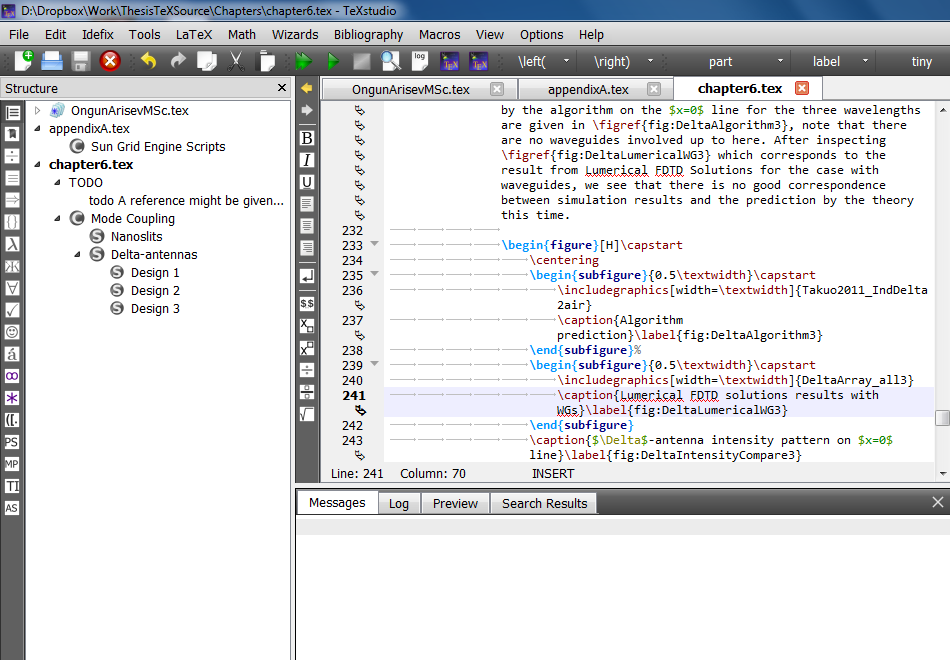
\includegraphics[width=0.99\linewidth]{res/images/latex.jpg}
			\caption{\TeX{}studio - per la stesura dei documenti}
		\end{figure} 
		\paragraph{Draw.io} \mbox{}\\ \mbox{}\\
		Draw.io, già citato in precedenza, viene utilizzato per la produzione degli UML\glo. \newline
		\centerline{\url{https://www.draw.io/}}
		
	\subsection{Gestione della configurazione}
	\subsubsection{Scopo}
	Lo scopo della configurazione è di creare ordine tra software e documenti. Tutto ciò che è configurato si trova in un posto preciso, ha uno stato identificativo, è modificato secondo procedure e posto sotto versionamento.
	\subsubsection{Versionamento}
	\paragraph{Codice di versione del documento} \mbox{}\\ \mbox{}\\
	Ogni documento, deve avere una storia, ricostruibile attraverso le sue versioni. Ogni versione deve corrispondere a una riga della tabella delle modifiche. Ogni numero di versione è composto da tre cifre:
	\begin{center}
		X.Y.Z
	\end{center}
	\begin{itemize}
		\item \textbf{X}: rappresenta una versione stabile del documento, resa tale dopo l' approvazione del responsabile di progetto:
		\begin{itemize}
			\item inizia da 0;
			\item viene incrementato dal responsabile di progetto all'approvazione del documento.
		\end{itemize}
		\item \textbf{Y}: rappresenta una versione parzialmente stabile del documento che è stata soggetta a verifica da parte di un verificatore:
		\begin{itemize}
			\item inizia da 0;
			\item viene incrementato dal verificatore ad ogni verifica;
			\item quando viene incrementato X, viene riportato a 0.
		\end{itemize}
		\item \textbf{Z}: rappresenta una versione instabile del documento in fase di lavorazione da parte dei redattori:
		\begin{itemize}
			\item inizia da 0;
			\item viene incrementato dal redattore del documento ad ogni modifica;
			\item quando viene incrementato Y, viene riportato a 0.
		\end{itemize}			
	\end{itemize}
	\paragraph{Tecnologie} \mbox{}\\ \mbox{}\\
	Per le parti del progetto da versionare si è scelto di usare il sistema di versionamento distribuito Git, usando il servizio di GitHub per ospitare la repository\glosp remota.
	\paragraph{Repository} \mbox{}\\ \mbox{}\\
	I membri del team possono interagire con il VCS (Version Control System) sia da linea di comando, sia attraverso software che ne migliorano l'usabilità, come GitFlow e GitKraken. La versione comune e ufficiale del progetto è ospitata in una repository\glosp remota su Github all'indirizzo: \newline \newline
	\centerline{\url{https://github.com/8LabSolutions/Soldino}}
	\paragraph{Struttura del repository} \mbox{}\\ \mbox{}\\
	Ci sono due tipi di repository\glo{}, la cui struttura è identica:
	\begin{itemize}
		\item \textbf{locale}: ogni membro del gruppo lavora sui file clonati dal repository\glo{} remoto nel proprio computer;
		\item \textbf{remoto}: pubblicato su GitHub, contiene il lavoro svolto da ogni componente e che viene condiviso con il team.
	\end{itemize}						
	Entrambe i tipi di repository\glosp sono organizzati in cartelle:
	\begin{itemize}
		\item \textbf{latex}: contiene tutti i file che definiscono il template \LaTeX{} per la creazione di un nuovo documento. Tra questi vi sono i file che definiscono i comandi personalizzati utilizzati dal gruppo e i package che devono essere inclusi per poter compilare i documenti;
		\item \textbf{guide}: cartella che contiene delle brevi guide di carattere pratico, come brevi spiegazioni per l'utilizzo dei comandi \LaTeX{} poco conosciuti;
		\item \textbf{script} cartella contenente script di utilità per il calcolo delle metriche;
		\item \textbf{01-RR}: raccoglie i file sorgenti per la compilazione dei documenti, suddivisi tra esterni ed interni, realizzati per la Revisione dei Requisiti;
		\item \textbf{01-RP}: raccoglie i file sorgenti per la compilazione dei documenti, suddivisi tra esterni ed interni, realizzati per la Revisione di Progettazione;
		\item Saranno aggiunte in futuro cartelle distinte nominate \textbf{03-RQ} e \textbf{04-RA} contenenti i file delle rispettive consegne.
	\end{itemize}
	La suddivisione dei file per revisione aiuta ad evidenziare il lavoro svolto per ogni consegna e migliora la tracciabilità dei file all'interno di ognuna di esse.
	\paragraph{Tipi di file e .gitignore} \mbox{}\\ \mbox{}\\
	I file utilizzati per la documentazione del progetto sono:
	\begin{itemize}
		\item file con estensione .tex di \LaTeX{};
		\item file con estensione .pdf che sono oggetto di consegna;
		\item alcuni file testuali e immagini di supporto ai precedenti.
	\end{itemize}			
	Il file ".gitignore" è presente al livello più esterno della repository\glosp ed elenca tutti i file da escludere dal versionamento. 
	\paragraph{Utilizzo di Git} \mbox{}\\ \mbox{}\\
	Il repository\glosp di Git è composto da vari branch, per lavorare in modo modulare e collaborativo.  
	Quindi viene consiglia questa procedura:
	\begin{enumerate}
		\item scegliere il branch su cui si vuole lavorare in base al compito assegnato;
		\item eseguire il pull dal repository\glosp remoto che effettua l'aggiornamento del proprio repository\glosp locale;
		\item svolgere il lavoro assegnato, che può consiste nell'aggiunta di nuovo materiale o nella modifica di file già presenti;
		\item eseguire il comando di aggiunta dei file nuovi o modificati da condividere all'area di staging\glo;
		\item eseguire il comando di commit dei file aggiunti, corredato da un messaggio che identifica il task eseguito;
		\item eseguire il push del commit sul repository\glosp remoto.
	\end{enumerate}
	\paragraph{Gestione delle modifiche} \mbox{}\\ \mbox{}\\
	Tutti i membri del team possono modificare i file in ogni branch, ad eccezione di quelli presenti nel branch master, per il quale occorre fare una pull request\glosp e ottenere l'approvazione di un altro membro .\newline
	Per effettuare modifiche maggiori sui contenuti o sulla struttura dei file è previsto di:
	\begin{itemize}
		\item contattare il responsabile del file da modificare;
		\item suggerire la modifica da effettuare;
		\item se il responsabile valuta positivamente la modifica, allora la applica.
	\end{itemize}
	Per modifiche minori, come correzioni grammaticali o miglioramenti sintattici, si consiglia di modificare indipendentemente.\newline
	In ambo i casi è opportuno commentare i propri commit con chiarezza per risalire facilmente alle modifiche.

\subsection{Gestione della qualità}
	\subsubsection{Scopo}
	Lo scopo è di garantire che il prodotto e i servizi offerti rispettino gli obiettivi di qualità e che i bisogni del proponente siano soddisfatti.
	\subsubsection{Aspettative}
	Attraverso la gestione della qualità si intende ottenere:
	\begin{itemize}
		\item qualità nell'organizzazione e nei suoi processi;
		\item qualità nel prodotto;
		\item qualità provata oggettivamente;
		\item soddisfazione finale di cliente e proponente.
	\end{itemize}
	\subsubsection{Descrizione}
	Per la trattazione approfondita della gestione della qualità si fa riferimento al \textit{Piano di Qualifica v2.0.0}, dove sono descritte le modalità utilizzate per garantire la qualità nello sviluppo del progetto. In particolare, in tale documento:
	\begin{itemize}
		\item sono presentati gli standard utilizzati;
		\item sono individuati i processi di interesse negli standard;
		\item sono individuati gli attributi del software più significativi per il progetto.
	\end{itemize}
	Per ogni processo vengono descritti:
	\begin{itemize}
		\item le metriche da utilizzare.
		\item gli intervalli entro i quali le misurazioni sono ritenute preferibili e accettabili.
	\end{itemize}
	L'obiettivo è di controllare e migliorare i processi e i loro 
	risultati.\newline
	Per ogni prodotto vengono descritti:
	\begin{itemize}
		\item gli obiettivi da perseguire;
		\item le metriche da utilizzare.
	\end{itemize}
	In questo caso si mira ad ottenere software e documentazione di qualità soddisfacente.
	\subsubsection{Attività}
	Le tre attività principali del processo sono:
	\begin{itemize}
		\item \textbf{Pianificazione}: porsi degli obiettivi di qualità, definire strategie per raggiungerli e disporre di conseguenza le persone e le risorse nel modo migliore;
		\item \textbf{Valutazione}: mettere in atto la pianificazione, applicando i criteri, misurando e monitorando i risultati; 
		\item \textbf{Reazione}: sulla base dei risultati, adattare le proprie strategie, criteri e piani.
	\end{itemize}
	\subsubsection{Strumenti}
	Gli strumenti predefiniti per la qualità sono: 
	\begin{itemize}
		\item i processi forniti dallo standard \textbf{ISO-12207};
		\item le metriche.
	\end{itemize}
\subsection{Verifica}
	\subsubsection{Scopo}
	Il processo di verifica ha per scopo la realizzazione di prodotti corretti, coesi e completi. Sono soggetti a verifica il software e i documenti. 
	\subsubsection{Aspettative}
	Il corretto svolgimento del processo di verifica rispetta i punti seguenti:	
	\begin{itemize}
		\item viene effettuata seguendo procedure definite;
		\item vi sono criteri chiari e affidabili da seguire per verificare;
		\item i prodotti passano attraverso fasi successive, ognuna delle quali è verificata;
		\item dopo la verifica il prodotto è in uno stato stabile;
		\item rende possibile la validazione.
	\end{itemize}
	\subsubsection{Descrizione}
	Il processo di verifica prende in input ciò che è già stato prodotto e lo restituisce in uno stato conforme alle aspettative. Per ottenere tale risultato ci si affida a processi di analisi e test.
	\subsubsection{Attività}
		\paragraph{Analisi} \mbox{}\\ \mbox{}\\
		Il processo di analisi si suddivide in statica e dinamica. \newline \newline
			\textbf{Analisi statica} \mbox{}\\ \mbox{}\\
			L'analisi statica effettua controlli su documenti e codice, di cui valuta e applica la correttezza (intesa come assenza di errori e difetti), la conformità a regole e la coesione\glosp dei componenti.\newline Per effettuare analisi statica esistono metodi manuali di lettura (attuati da persone) e metodi formali (attuati da macchine). Quelli manuali sono due:
			\begin{itemize}
				\item \textbf{Walkthrough}: i vari componenti del team analizzano gli oggetti nella loro totalità per cercare anomalie, senza sapere inizialmente se vi siano difetti, quali e dove siano;
				\item \textbf{Inspection}: i verificatori usano liste di controllo per fare ispezione cercando errori specifici in parti specifiche.
			\end{itemize}
			A seguire sono descritte le liste di controllo utilizzabili per le ispezioni. Si prevede l'ampliamento delle viste al progredire delle stesse ispezioni e degli errori trovati.
%\begin{comment}
			\begin{table}[H]
				\centering\renewcommand{\arraystretch}{1.5}
				\arrayrulecolor{white}
				\caption{Errori frequenti nei documenti}
				\begin{tabular}{c|c}
					
					\rowcolorhead
					{\colorhead \textbf{Oggetto}} &
					{\colorhead \textbf{Controllo} }\\
					
					\rowcolorlight
					{\colorbody Formato data} & {\colorbody Deve seguire il formato americano \textit{YYYY-MM-DD}} 
					\\
					
					\rowcolordark
					{\colorbody Sintassi} & {\colorbody  La frase è troppo complessa e può essere semplificata } 
					\\	
					
					\rowcolorlight
					{\colorbody Parte mancante} & {\colorbody Controllare titoli vuoti o sezioni di grandezza insolita} 
					\\
					
					\rowcolordark
					{\colorbody Forma dei verbi} & {\colorbody In generale è preferibile il presente indicativo} 
					\\
					
					\rowcolorlight
					{\colorbody Punteggiatura degli elenchi} & {\colorbody Ogni voce termina in \textbf{";"} eccetto l'ultima che termina in \textbf{"."}} 
					\\
				\end{tabular}
			\end{table}
%\end{comment}
			% PLACEHOLDER: lista di ispezione del codice, da aggiungere quando si fa il codice.				
			\mbox{}\\								
			\textbf{Analisi dinamica} \mbox{}\\ \mbox{}\\
			L'analisi dinamica è una tecnica di analisi del prodotto software che richiede la sua esecuzione. Viene effettuata  mediante dei test che verificano se il prodotto funziona e se ci sono anomalie. 
			
		\paragraph{Test} \mbox{}\\ \mbox{}\\
		I test sono l'attività fondamentale dell'analisi dinamica: il loro scopo è verificare che il codice scritto funzioni correttamente.
		Per ogni test devono essere definiti i seguenti parametri:
		\begin{itemize}
			\item \textbf{ambiente}: sistema hardware e software sul quale verrà eseguito il test;
			\item \textbf{stato iniziale}: lo stato iniziale dal quale il test viene eseguito;
			\item \textbf{input}: input inserito;
			\item \textbf{output}: output atteso;
			\item \textbf{istruzioni aggiuntive}: ulteriori istruzioni su come va eseguito il test e su come vanno interpretati i risultati ottenuti.
		\end{itemize}
		Test ben scritti devono:
		\begin{itemize}
			\item essere ripetibili;
			\item specificare l'ambiente di esecuzione;
			\item identificare input e output richiesti;
			\item avvertire di possibili effetti indesiderati;
			\item fornire informazioni sui risultati dell'esecuzione in forma di file di log.
		\end{itemize}	
			
		\noindent{Ci sono vari tipi di test del software, ognuno dei quali ha un diverso oggetto di verifica e scopo. La codifica dei seguenti test è presente nel documento \textit{Norme di Progetto v2.0.0}.}
		
		%\subsection{Tipi di test}
		%Vengono individuate quattro tipologie di test:
		\begin{itemize}
			\item \textbf{Test di Accettazione[TA]}: anche detto "test di collaudo", è simile al test di sistema per l'oggetto testato, ma viene eseguito con la collaborazione dei committenti. Si occupa di verificare il prodotto e, in particolare, il soddisfacimento del cliente. Il superamento del test di collaudo garantisce che il software sia pronto per essere rilasciato. Tali test verranno indicati nel seguente modo: \\
			\centerline{\textbf{TA[Tipo][Importanza][Codice]}}
			dove:
			\begin{itemize}
				\item \textbf{Tipo}: indica di che tipo si tratta il requisito. Può
				appartenere a una delle seguenti categorie indicate con:
				\begin{itemize}
					\item \textbf{O} per i requisiti obbligatori;
					\item \textbf{D} per i requisiti desiderabili;
					\item \textbf{F} per i requisiti facoltativi.			
				\end{itemize}
				\item \textbf{Importanza}: indica l'importanza del requisito. L'importanza
				che può assumere un requisito viene indicata con:
				\begin{itemize}
					\item \textbf{F} per indicare un requisito funzionale;
					\item \textbf{V} per indicare un requisito di vincolo;
					\item \textbf{Q} per indicare un requisito di qualità;
					\item \textbf{P} per indicare un requisito prestazionale. 
				\end{itemize}
				\item \textbf{Codice}: rappresenta il codice identificativo crescente
				del componente da verificare.
			\end{itemize}
			\item \textbf{Test di Sistema [TS]}: il sistema viene testato nella sua interezza, una volta integrati tutti i suoi componenti. Ci si concentra sulle interazioni tra le parti, sul comportamento emergente\glosp delle caratteristiche del sistema e sulla copertura\glosp di tutte le funzionalità. Questo tipo di test porta alla luce le ipotesi errate che i diversi sviluppatori fanno su parti del software sviluppate da altri.
			In questa fase ci si assicura che il sistema rispetti tutte le specifiche definite nell'\textit{Analisi dei Requisiti}. Tali test verranno indicati nel seguente modo:\\
			\centerline{\textbf{TS[id]}}
			dove \textit{id} rappresenta il codice identificativo crescente del componente da
			verificare.\\
			Tale tipologia di test verrà sviluppata in un immediato futuro, in seguito alla richiesta della sua istanziazione;
			\item \textbf{Test di Integrazione [TI]}: dopo aver superato i test di unità, le stesse unità vengono assemblate in agglomerati progressivamente più grandi. Il test di integrazione si concentra sulle interfacce tra i componenti. Un agglomerato che supera il test di integrazione costituisce quindi una nuova unità per un agglomerato di grandezza maggiore. Questa procedura si ripete fino a raggiungere la dimensione totale del sistema. Tali test verranno indicati nel seguente modo:\\
			\centerline{\textbf{TI[id]}}
			dove \textit{id} rappresenta il codice identificativo crescente del componente da
			verificare.\\
			Tale tipologia di test verrà sviluppata in un immediato futuro, in seguito alla richiesta della sua istanziazione;
			\item \textbf{Test di Unità [TU]}: si eseguono su unità di software. Questi test si concentrano sul funzionamento delle unità individuali. Dati gli input possibili in un unità, si suddividono gli input in partizioni di equivalenza e si prova se gli input attesi danno gli output previsti. Le singole unità possono essere testate con l'ausilio di driver\glosp e stub\glo. Tali test verranno indicati nel
			seguente modo:\\
			\centerline{\textbf{TU[id]}}
			dove \textit{id} rappresenta il codice identificativo crescente dell'unità da verificare.\\
			Tale tipologia di test verrà sviluppata in un immediato futuro, in seguito alla richiesta della sua istanziazione.
			\item \textbf{Test di regressione}: Si effettua di seguito ad una modifica del sistema e consiste nella riesecuzione dei test esistenti: si combina bene con l'automazione dei test.
		\end{itemize}
		
		
			%\textbf{Test di unità} \mbox{}\\ \mbox{}\\
			% \newline \newline
			%\textbf{Test di integrazione} \mbox{}\\ \mbox{}\\
			% \newline \newline
			%\textbf{Test di sistema} \mbox{}\\ \mbox{}\\
			% \newline \newline
			%\textbf{Test di regressione} \mbox{}\\ \mbox{}\\
			% \newline \newline
			%\textbf{Test di accettazione} \mbox{}\\ \mbox{}\\
			
	\subsubsection{Strumenti}
		\paragraph{Verifica ortografica} \mbox{}\\ \mbox{}\\
		Viene utilizzata la verifica dell'ortografia in tempo reale, strumento integrato in \TeX{}studio che sottolinea in rosso le parole errate e in verde le ripetizioni a breve distanza secondo la lingua italiana.
		\paragraph{Validazione W3C} \mbox{}\\ \mbox{}\\
		Per la validazione delle pagine di markup HTML viene utilizzato lo strumento offerto dal W3C, raggiungibile al seguente indirizzo: \newline
		\centerline{\url{https://validator.w3.org/}} \newline \newline
		Per la validazione dei fogli di stile CSS viene utilizzato lo strumento offerto dal W3C, raggiungibile al seguente indirizzo: \newline
		\centerline{\url{https://jigsaw.w3.org/css-validator/}} \newline


\subsection{Validazione}
	\subsubsection{Scopo}
	Lo scopo della validazione è stabilire se il prodotto soddisfa il compito per cui è stato creato. Dopo la validazione, è garantito che il software rispetti i requisiti e che soddisfi i bisogni del committente.
	\begin{comment}
	\subsubsection{Aspettative}
	Una corretta implementazione di questo processo permette di individuare:
	\begin{itemize}
		\item una procedura di validazione;
		\item i criteri per la validazione del prodotto;
		\item le conformità del prodotto finito.
	\end{itemize}
	\end{comment}
	\subsubsection{Descrizione}
	\`E compito dei progettisti definire la pianificazione e la progettazione dei test, mentre è compito dei verificatori eseguirli e tracciarne i risultati tramite gli strumenti stabiliti.
	\subsubsection{Attività}
	Per validare il prodotto si devono rispettare i seguenti punti:
	\begin{itemize}
		\item identificare gli oggetti da validare;
		\item identificare una strategia con delle procedure di validazione in cui le procedure di verifica possono essere riutilizzare;
		\item applicare la strategia;
		\item valutare che i risultati rispettino le aspettative.
	\end{itemize}
	Questo processo si può suddividere in due attività principali:
	\begin{itemize}
		\item \textbf{Test di sistema}
		\item \textbf{Test di accettazione}
	\end{itemize}
	I test di sistema sono eseguiti tramite test di integrazione che non verificano la conformità rispetto alle attese delle funzionalità presenti. Per avere la totale certezza del soddisfacimento di tutti requisiti i test di accettazione verranno tracciati in modo automatico utilizzando lo strumento PragmaDB.
	
	

\subsection{Metriche di qualità}
\subsubsection{Documentazione}
La documentazione consiste nella produzione di informazioni, la cui forma tipica è documentale, e nella loro gestione. I documenti sono prodotti a supporto di tutte le attività di progetto.
L'obiettivo è di scrivere la documentazione affinché costituisca una body of knowledge\glosp che raccoglie la conoscenza in modo:
\begin{itemize}
	\item completo;
	\item non ambiguo;
	\item modulare e fatto di parti coese;
	\item trasparente, adatto alla trasmissione delle informazioni;
	\item disponibile esternamente.
\end{itemize}
La strategia prevede che i documenti siano: 
\begin{itemize}
	\item prodotti in concomitanza con tutte le attività di sviluppo;
	\item prodotti in modo collaborativo;
	\item supportati da un glossario;
	\item supportati dalle Norme di Progetto;
	\item prodotti con strumenti software adatti alla collaborazione e alla modularità in \LaTeX;
	\item ospitati in una repository\glosp pubblica su GitHub.
\end{itemize}
Le metriche utilizzate sono:
\begin{itemize}
	\item l'\textbf{indice di Gulpease}, ossia un indice che indica la leggibilità del testo. Si misura con la seguente formula:
	\begin{center}
		$I_G = 89+ \frac{(300 \cdot numero\ di\ frasi - 10 \cdot numero\ di\ lettere)}{numero\ di\ parole}$;
	\end{center}
	\item il numero di errori ortografici o grammaticali.
\end{itemize}
	\subsubsection{Pianificazione}
La pianificazione è un'attività significativa della gestione di progetto. Consiste nel governare le	risorse a disposizione, ovvero tempi, costi e ruoli, monitorarle nel tempo e reagire efficacemente ai cambiamenti. La pianificazione si esprime specificatamente all'interno del \textit{Piano di Progetto}.\\
Gli obiettivi sono:
\begin{itemize}
	\item avere a disposizione piani e obiettivi ben definiti;
	\item aver definito ruoli, responsabilità, obblighi e autorità a cui rispondere;
	\item aver allocato le risorse e i beni necessari;
	\item attivare il piano per sostenere il progetto.
\end{itemize}
La strategia prevede di: 
\begin{itemize}
	\item produrre la pianificazione delle attività;
	\item mantenerla aggiornata mentre esse vengono svolte;
	\item usarla come riferimento e supporto.
\end{itemize}
Le metriche utilizzate sono:
\begin{itemize}
	\item \textbf{Actual Cost} (AC): il denaro speso fino al momento del calcolo;
	\item \textbf{Earned Value} (EV): metrica di utilità per il calcolo di $SV$ e $CV$ (spiegate successivamente). Si tratta del valore del lavoro fatto fino al momento del calcolo; corrisponde al denaro guadagnato fino a quel momento;
	\item \textbf{Planned Value} (PV): metrica di utilità per il calcolo di $SV$ e $CV$ (spiegate successivamente). Si tratta del valore del lavoro pianificato al momento del calcolo: corrisponde al denaro che si dovrebbe aver guadagnato in quel momento. Si misura con $BAC \cdot \%\ di\ lavoro\ pianificato\ $;
	\item \textbf{Schedule Variance} (SV): Esprime lo stato di anticipo o ritardo nello svolgimento del progetto rispetto alla pianificazione. Si calcola come $SV = EV - PV$
	\item \textbf{Cost Variance} (CV): Differenza tra il costo del lavoro effettivamente completato e quello
	pianificato. Una CV positiva indica che si sta rispettando il budget. Si calcola come $CV = EV - AC$;
\end{itemize}
\subsubsection{Verifica}
Il processo consiste nella ricerca e correzione di anomalie e difetti nei processi e prodotti del	progetto, mediante tecniche predefinite e se possibile automatiche.\\
Gli obiettivi sono:
\begin{itemize}
	\item individuare e correggere le anomalie;
	\item provare che il sistema soddisfi i requisiti.
\end{itemize}
La strategia prevede di: 
\begin{itemize}
	\item individuare tecniche e strumenti di verifica;
	\item applicarli;
	\item affinarli con l'esperienza.
\end{itemize}
La metrica utilizzata è la \textbf{Code Coverage} (CC), una percentuale che indica il numero di righe di codice percorse dai test durante la loro	esecuzione. Per linee di codice totali si intende tutte quelle appartenenti all'unità in fase di test e si calcola con la seguente formula:
\begin{center}
	$CC = \frac{linee\ di\ codice\ percorse}{linee\ di\ codice\ totali}$
\end{center}



	\pagebreak
	
	\section{Processi Organizzativi}
	\subsection{Gestione Organizzativa}
		\subsubsection{Scopo}
		Il processo di gestione contiene le attività di carattere gestionale. Queste attività consistono principalmente nell'istanziare processi nel progetto, pianificare e stimare tempi e costi, assegnare ruoli e rispettivi compiti ai membri del team, nonché controllare l'esecuzione e i risultati di tutti i processi in atto. La gestione compete al Responsabile di Progetto, che ha il compito di gestire il progetto, i suoi processi, i suoi prodotti e i membri del team.
		\subsubsection{Aspettative}
		Gli obiettivi di questo processo sono:
		\begin{itemize}
			\item Ottenere una pianificazione ragionevole delle attività da seguire;
			\item Coordinare i membri del team assegnando loro ruoli, compiti e facilitando la comunicazione tra loro;
			\item Adoperare processi per regolare le attività e renderle economiche;
			\item Mantenere il controllo sul progetto in modo efficace ma non invasivo, monitorando il team, i processi e i prodotti.
		\end{itemize}
		\subsubsection{Descrizione}
		Le attività di gestione seguono il flusso di fasi seguente:
		\begin{itemize}
			\item inizio e definizione dello scopo;
			\item pianificazione;
			\item esecuzione e controllo;
			\item revisione e valutazione;
			\item chiusura.
		\end{itemize}
		\subsubsection{Ruoli di progetto}
		Ciascun membro del gruppo, a rotazione, si impegnerà a ricoprire i  ruoli che corrispondono alle omonime figure aziendali. Nel Piano di Progetto vengono organizzate e pianificate le attività assegnate ai specifici ruoli previsti nell'attività di progetto. I ruoli che ogni componente del gruppo è tenuto a rispettare sono descritti di seguito.
			\paragraph{Responsabile di progetto} \mbox{}\\
			Il responsabile di progetto è una figura importante in quanto ricadono su di lui le responsabilità di pianificazione, gestione, controllo e coordinamento. Un altro ruolo del responsabile è quello di rappresentare l'interfaccia del gruppo con le persone esterne ad esso: sono quindi di sua competenza le comunicazioni con committente e proponente. \\
			Il responsabile deve quindi:
			\begin{itemize}
				\item gestire, controllare e coordinare risorse e attività del gruppo;
				\item  gestire, controllare e coordinare gli altri componenti del gruppo;
				\item analizzare e gestire le criticità;
				\item approvare i documenti.
			\end{itemize}
			\paragraph{Amministratore di progetto} \mbox{}\\
			L'amministratore ha il compito di supporto e controllo dell'ambiente di lavoro. \\
			L'amministratore deve quindi:
			\begin{itemize}
				\item amministrazione delle infrastrutture di supporto;
				\item risoluzione dei problemi legati alla gestione dei processi;
				\item gestione della documentazione;
				\item controllo di versioni e configurazioni.
			\end{itemize}
			\paragraph{Analista} \mbox{}\\
			L'analista si occupa di analisi dei problemi e del dominio applicativo. Questa figura non sarà sempre presente durante il progetto. \\
			L'analista deve quindi:
			\begin{itemize}
				\item studio del dominio del problema e del problema stesso, definendone complessità e requisiti;
				\item redazione di Analisi dei Requisiti e Studio di Fattibilità.
			\end{itemize}
			\paragraph{Progettista} \mbox{}\\
			Il progettista gestisce gli aspetti tecnologici e tecnici del progetto.\\
			Il progettista deve:
			\begin{itemize}
				\item effettuare scelte efficienti ed ottimizzate su aspetti tecnici del progetto;
				\item sviluppare un'architettura che sfrutti tecnologie note ed ottimizzate su cui basare un prodotto stabile e mantenibile.
			\end{itemize}
			\paragraph{Programmatore} \mbox{}\\
			Il programmatore è il responsabile della codifica del progetto e delle componenti di supporto, che serviranno per effettuare le prove di verifica e validazione sul prodotto.\\
			Il programmatore deve:
			\begin{itemize}
				\item implementare le decisioni del progettista;
				\item creare o gestire componenti di supporto per la verifica e la validazione del codice.
			\end{itemize}
			\paragraph{Verificatore} \mbox{}\\
			Il verificatore si occupa di controllare il prodotto del lavoro svolto dagli altri membri del team, sia esso codice o documentazione. Per le correzioni si affida agli standard definiti nelle Norme di Progetto, nonché alla propria esperienza e capacità di giudizio.\\
			Il verificatore deve:
			\begin{itemize}
				\item ispezionare i prodotti in fase di revisione, avvalendosi delle tecniche e degli strumenti definiti nelle NdP;
				\item correggere difetti ed errori del prodotto in esame;
				\item decidere se applicare le correzioni in autonomia o in collaborazione con l'autore del prodotto in questione, a seconda della natura dell'errore.
			\end{itemize}
		\subsubsection{Procedure}
		Seguono le modalità che il gruppo adotterà durante la realizzazione del progetto. Le comunicazioni saranno interne, ossia coinvolgono i partecipanti del gruppo, o esterne, ossia coinvolgono anche proponente e committente.
			\paragraph{Gestione delle comunicazioni} \mbox{}\\
			\subparagraph{Comunicazioni interne} \mbox{}\\
			Le comunicazioni interne al gruppo avvengono utilizzando Slack. Slack è un software di collaborazione aziendale adatto al lavoro di gruppo: permette di separare i vari argomenti di discussione in canali e i team in workspace; permette anche di integrare servizi di terze parti utili al team, tra cui bot e chiamate. Le sue funzionalità e la sua conformità agli scopi del progetto ne hanno favorito la scelta.
			\subparagraph{Comunicazioni esterne} \mbox{}\\
			Le comunicazioni con soggetti esterni al gruppo sono di competenza del responsabile. Gli strumenti predefiniti sono la posta elettronica, che utlizza l'indirizzo 8labsolutions@gmail.com creata in fase di creazione del team e, su suggerimento del proponente, un canale Slack creato proprio da Red Babel. Il responsabile ha il compito di tenere informati gli altri componenti del gruppo.
			\paragraph{Gestione degli incontri} \mbox{}\\
			\subparagraph{Incontri interni del team} \mbox{}\\
			Le riunioni interne del team sono organizzate dal responsabile in accordo con i membri del team. Per stabilire data e ora viene utilizzato Google Calendar, dove ogni membro segnala gli orari nel quale ha impegni.
			\subparagraph{Verbali di riunioni interne} \mbox{}\\
			Ad ogni riunione interna fatta corrisponderà un verbale. Questo sarà redatto da segretario, persona nominata dal responsabile, che dovrà tenere nota delle discussioni fatte e delle decisioni prese. 
			\subparagraph{Incontri esterni del team} \mbox{}\\
			Il responsabile ha il compito di comunicare e organizzare gli incontri con  proponente e committente. Se un membro del gruppo, il proponente o il committente ritiene necessario organizzare un incontro il responsabile decide una data, in accordo tra le due parti, e la comunica tramite i canali sopra citati.\newline Le riunioni esterne sono di grande importanza per la buona riuscita del progetto: a esse si presta molta cura.
			\subparagraph{Verbali esterni di riunione} \mbox{}\\
			Come per le riunioni interne, anche per le esterne viene redatto un verbale. La struttura dei due tipologie è analoga, ma essendo le riunioni esterne di maggiore criticità, il verbale va redatto con maggiore attenzione, evitando di tralasciare informazioni importanti.
			\paragraph{Gestione degli strumenti di coordinamento} \mbox{}\\
			\subparagraph{Tickecting} \mbox{}\\
			Il ticketing consente ai membri di avere chiaro in ogni momento quali attività sono in corso; permette al RdP di assegnare compiti ai membri del team e di controllare l'andamento delle attività; permette ai membri del team di conoscere e gestire il proprio carico di lavoro.\newline Lo strumento di ticketing scelto è Trello: consiste in una lavagna virtuale online dove ogni task corrisponde a un compito, a cui sono associati una data di scadenza e un insieme di membri assegnatari. Ogni compito passa attraverso i seguenti stati:
			\begin{itemize}
			\item da fare;
			\item in lavorazione;
			\item in revisione;
			\item completato.
			\end{itemize}
			La scelta di Trello è stata determinata dalla sua facilità di apprendimento, di controllo, dall'usabilità e dalla trasparenza che fornisce. La gestione dei ticket dev'essere scrupolosa, perché la lavagna di Trello tende ad affollarsi velocemente.
			\paragraph{Gestione degli strumenti di versionamento} \mbox{}\\
			\subparagraph{Repository} \mbox{}\\
			Il sistema di versionamento usato è \textit{Git}, noto sistema di controllo versione distribuito. I membri del team possono usare lo strumento sia da linea di comando sia attraverso software che ne migliorano l'usabilità, come GitFlow, GitKraken. La versione comune e ufficiale del progetto è  ospitata in una repository remota su Github all'indirizzo  
			\url{https://github.com/8LabSolutions/Soldino}. Questa repository remota è pubblica quindi accessibile a tutti, inclusi cliente e committente.
			\subparagraph{Struttura del repository} \mbox{}\\
			Ci sono due tipi di repository:
			\begin{itemize}
				\item remota: ospitata su \textit{GitHub}, è la versione di riferimento e quella disponibile all'esterno del team;
				\item locale: ogni studente possiede una copia locale del progetto su cui lavorare;
			\end{itemize}						
			Entrambe i tipi di repository sono organizzati in cartelle:
			\begin{itemize}
				\item latex: qui risiedono i file di carattere generale, come i file relativi a package, che vengono inseriti in tutti i documenti, e i template, che sono usati come riferimento per nuovi documenti di struttura già definita;
				\item guide: qui si trovano delle brevi guide di carattere pratico, come brevi spiegazioni per applicare comandi latex poco conosciuti;
				\item \textit{RR}: qui si trovano i documenti, suddivisi tra esterni ed interni, la cui consegna è dovuta alla Revisione dei Requisiti;
				\item Saranno aggiunte in futuro cartelle distinte nominate \textbf{RP}, \textbf{RQ} e \textbf{RA} contenenti i file delle rispettive consegne.
			\end{itemize}
			Lo scopo della suddivisione dei file per revisioni è di evidenziare il lavoro svolto per ogni milestone maggiore, e di rendere ben tracciabili i file che le riguardano.
			\subparagraph{Tipi di file e .gitignore} \mbox{}\\
			I file di interesse per il progetto sono:
			\begin{itemize}
				\item file .tex di \LaTeX{};
				\item file .pdf che sono oggetto di consegna;
				\item alcuni file testuali e immagini di supporto ai precedenti.
			\end{itemize}			
			Il file .gitignore presente al livello più esterno della repository elenca ed esclude tutti i file che vengono prodotti durante lo sviluppo del progetto ma non sono rilevanti per la consegna.
			\subparagraph{Lavoro collaborativo e versionamento} \mbox{}\\
			La repository \textit{git} è composta di vari rami per organizzare il lavoro e renderlo modulare e collaborativo. Ogni membro del team lavora in locale su un branch della repository; si può lavorare in più su uno stesso ramo; è auspicabile lavorare parallelamente su rami differenti a diverse attività parallele.\newline La sequenza di attività che un membro del team usa produrre un incremento da aggiungere al progetto è la seguente:
			\begin{enumerate}
				\item scelta del branch corretto;
				\item pull dalla repository remota per aggiornare il proprio branch locale;
				\item svolgimento del lavoro, che risulta nella modifica dei propri file locali;
				\item aggiunta dei file al sistema di versionamento;
				\item commit dei file aggiunti, corredato di un messaggio che identifica le modifiche;
				\item push del commit nella repository remota;
			\end{enumerate}
			La routine serve a massimizzare la consistenza e minimizzare i conflitti tra le repository locali e quelle remote, così da rendere il lavoro il più possibile piacevole e snello.

			\paragraph{Gestione dei rischi} \mbox{}\\
			Il Responsabile di Progetto ha il compito di rilevare i rischi e manutenerli, documentando quest'attività nel Piano di Progetto. La procedura da seguire per la gestione dei rischi è la seguente:
			\begin{itemize}
				\item individuare nuovi problemi e monitorare i rischi già previsti;
				% PLACEHOLDER: sostituire la frase sottostante, in particolare 'riscontro'
				\item registrare ogni riscontro previsto dei rischi nel Piano di Progetto;
				\item aggiungere i nuovi rischi individuati nel Piano di Progetto;
				\item ridefinire, se necessario, le strategie di progetto.
			\end{itemize}
				\subparagraph{Codifica dei rischi}
				Le tipologie di rischi sono così codificate:
				\begin{itemize}
					\item \textbf{RT}: Rischi Tecnologici;
					\item \textbf{RO}: Rischi Organizzativi;
					\item \textbf{RI}: Rischi Interpersonali.
				\end{itemize}
			\paragraph{Gestione di progetto}
			Per dividere le attività da svolgere e per assicurarsi che tutto venga svolto entro una deadline si è scelto di utilizzare Trello. Questo permette di assegnare una specifica attività ad un membro e impostare anche una scadenza entro la quale l'attività dovrà essere terminata. Sarà il responsabile a gestire la suddivisione degli incarichi tra i membri e a determinare le scadenze per queste.
		\subsubsection{Strumenti utilizzati}
		Il gruppo, nel corso del progetto, ha utilizzato o utilizzerà i seguenti strumenti:
		\begin{itemize}
			\item \textbf{Telegram}: strumento di messaggistica utilizzato per un'iniziale gestione del gruppo;
			\item \textbf{Slack}: per la comunicazione interna del team ed eventuali comunicazioni col proponente;
			\item \textbf{Trello}: per assegnare determinate attività e imporre una scadenza;
			\item \textbf{Git}: sistema di controllo di versionamento;
			\item \textbf{Gitflow, GitKraken}: interfacce per utilizzare Git più comodamente sul proprio desktop;
			\item \textbf{GitHub}: per il versionamento e il salvataggio in remoto di tutti i file riguardanti il progetto.
			\item \textbf{Google Drive e Documenti}: utilizzato per la stesura di file che sono soggetti a molti cambiamenti e devono essere visibili a tutti nella sua versione più aggiornata come ad esempio il glossario;
			\item \textbf{Google Calendar}: per facilitare il lavoro al responsabile ogni settimana ciascun membro indica quando non è disponibile per un incontro;
			\item \textbf{Skype}: servizio che offre possibilità di fare video conferenze e chiamate VoIP, utilizzato per il primo contatto con il proponente;
			\item \textbf{Sistemi operativi}: i requisiti non indicano la necessità di usare un sistema operativo specifico, verranno quindi utilizzati sia Windows, sia Linux, sia Mac OS dai diversi membri del team; %niente mac perché viva la povertà!
		\end{itemize}
	\subsection{Formazione del team}
	Per quando riguarda l'apprendimento basilare delle tecnologie richieste per il progetto, il gruppo ha optato per l'auto-formazione. Le conoscenze acquisite sono condivise in maniera informale e consolidate o migliorate; le conoscenze più critiche sono condivise anche in forma scritta: nella repository si trovano infatti una Wiki per gli argomenti più comune e la cartella guide per alcune utilità pratiche minori. In caso di membri del team in difficoltà, i membri più esperti offrono spiegazioni, riferimenti o chi ne ha bisogno.			
	\pagebreak
	
	\appendix
	\section{Standard di qualità}

	\subsection{ISO/IEC 9126}
	ISO/IEC 9126 è uno standard internazionale per valutare la qualità del software.\\%PLACEHOLDER mettere eventuale immagine dello standard
	Questo standard è diviso in quattro parti:
	\begin{itemize}
		\item \textbf{Modello della qualità del software} (descritto dopo le successive 3 parti)
		\item \textbf{Metriche per la qualità interna}:metriche che si applicano al software non eseguibile durante le fasi di progettazione e codifica. Permettono di individuare eventuali problemi che potrebbero influire sulla qualità finale del prodotto prima che venga realizzato un eseguibile. Grazie alle misure effettuate tramite le metriche interne è possibile prevedere il livello di qualità esterna e di qualità in uso del prodotto finale, poiché entrambe vengono influenzate dalla qualità interna.\\
Viene rilevata tramite analisi statica. Idealmente la qualità interna determina la qualità esterna;
		\item \textbf{Metriche per la qualità esterna}: metriche applicabili al software in esecuzione che ne misurano il comportamento attraverso dei test, in funzione degli obiettivi stabiliti.\\
Viene rilevata tramite analisi dinamica. Idealmente la qualità esterna determina la qualità in uso;
		\item \textbf{Metriche per la qualità in uso}: metriche applicabili solo al prodotto finito ed in uso in condizioni reali.\\
La qualità in uso viene raggiunta solo se è stato raggiunto il livello di qualità interna e di qualità esterna.
	\end{itemize}
	Il modello di qualità del software, presentato nella prima parte dello standard, suddivide la qualità in sei caratteristiche generali e varie sotto caratteristiche, misurabili attraverso delle metriche, utilizzate per fornire una scala ed un metodo per la misurazione. Ecco l'elenco delle caratteristiche:
	\begin{itemize}
		\item \textbf{Funzionalità}: capacità del software di soddisfare i requisiti, descritti nell'Analisi dei Requisiti, in un determinato contesto.\\
Nello specifico il software deve soddisfare le seguenti caratteristiche:
		\begin{itemize}
			\item \textbf{Appropriatezza}: capacità di fornire funzioni appropriate per attività specifiche, che permettano di raggiungere gli obiettivi prefissati;
			\item \textbf{Accuratezza}: capacità di fornire i risultati concordati o la precisione richiesta;
			\item \textbf{Interoperabilità}: capacità di interagire ed operare con uno o più sistemi specificati;
			\item \textbf{Conformità}: capacità di aderire a standard;
			\item \textbf{Sicurezza}: capacità di proteggere informazioni e dati.
		\end{itemize}
\item \textbf{Affidabilità}: capacità del software di mantenere uno specifico livello di prestazioni quando usato in condizioni specificate.\\
Nello specifico il software deve soddisfare le seguenti caratteristiche:
		\begin{itemize}
			\item \textbf{Maturità}: capacità di evitare il verificarsi di errori, malfunzionamenti o risultati non corretti;
			\item \textbf{Tolleranza agli errori}: capacità di mantenere livelli prefissati di prestazioni anche in presenza di malfunzionamenti o usi scorretti del prodotto finale;
			\item \textbf{Recuperabilità}: capacità di ripristinare un livello appropriato di prestazioni o di recupero di informazioni rilevanti a seguito di un malfunzionamento;
			\item \textbf{Aderenza}:  capacità di aderire a standard, regole e convenzioni che riguardano l'affidabilità.
		\end{itemize}
\item \textbf{Efficienza}: capacità del prodotto software di eseguire le proprie funzioni minimizzando il tempo necessario e sfruttando al meglio le risorse che necessita.\\
Nello specifico il software deve soddisfare le seguenti caratteristiche:
		\begin{itemize}
			\item \textbf{Nel tempo}: capacità di fornire adeguati tempi di risposta, elaborazione e velocità di attraversamento in determinate condizioni;
			\item \textbf{Nello spazio}: capacità di utilizzo di quantità e tipo di risorse in maniera adeguata;
		\end{itemize}
\item \textbf{Usabilità}: capacità del prodotto software di essere compreso, appreso, usato e accettato dall'utente, quando usato sotto determinate condizioni.\\
Nello specifico il software deve soddisfare le seguenti caratteristiche:
		\begin{itemize}
			\item \textbf{Comprensibilità}: capacità di essere chiaro riguardo le proprie funzionalità e il proprio utilizzo;
			\item \textbf{Apprendibilità}: capacità di essere facilmente apprendibile dagli utenti;
			\item \textbf{Operabilità}: capacità di permettere all'utente di eseguire i suoi scopi e controllarne l'uso;
			\item \textbf{Attrattività}: capacità di essere piacevole all'utente che l'utilizza.
		\end{itemize}
\item \textbf{Manutenibilità}: capacità del software di essere modificato, al fine di aggiungere correzioni, miglioramenti o adattamenti.\\
Nello specifico il software deve soddisfare le seguenti caratteristiche:
		\begin{itemize}
			\item \textbf{Analizzabilità}: capacità di essere facilmente analizzato al fine di localizzare un errore;
			\item \textbf{Modificabilità}: capacità di poter essere agevolmente modificato nel codice, nella progettazione o nella documentazione;
			\item \textbf{Stabilità}: capacità di evitare effetti indesiderati a seguito di una modifica;
			\item \textbf{Testabilità}: capacità di essere facilmente testato per validare le modifiche apportate.
		\end{itemize}
\item \textbf{Portabilità}: capacità del software di essere trasportato da un ambiente di lavoro ad un altro, sia esso hardware che software.\\
Nello specifico il software deve soddisfare le seguenti caratteristiche:
		\begin{itemize}
			\item \textbf{Adattabilità}: capacità di essere facilmente adattato a differenti ambienti operativi, senza applicare modifiche;
			\item \textbf{Installabilità}: capacità di poter essere installato in un determinato ambiente;
			\item \textbf{Conformità}: capacità di coesistere con altre applicazioni e di condividere risorse;
			\item \textbf{Sostituibilità}: capacità di essere utilizzato al posto di un altro software per svolgere gli stessi compiti, nello stesso ambiente.
		\end{itemize}
	\end{itemize}

	
	
\end{document}
